%% 11/23/2015
%%%%%%%%%%%%%%%%%%%%%%%%%%%%%%%%%%%%%%%%%%%%%%%%%%%%%%%%%%%%%%%%%%%%%%%%%%%%
% AGUJournalTemplate.tex: this template file is for articles formatted with LaTeX
%
% This file includes commands and instructions
% given in the order necessary to produce a final output that will
% satisfy AGU requirements. 
%
% You may copy this file and give it your
% article name, and enter your text.
%
%%%%%%%%%%%%%%%%%%%%%%%%%%%%%%%%%%%%%%%%%%%%%%%%%%%%%%%%%%%%%%%%%%%%%%%%%%%%
% PLEASE DO NOT USE YOUR OWN MACROS
% DO NOT USE \newcommand, \renewcommand, or \def, etc.
%
% FOR FIGURES, DO NOT USE \psfrag or \subfigure.
% DO NOT USE \psfrag or \subfigure commands.
%%%%%%%%%%%%%%%%%%%%%%%%%%%%%%%%%%%%%%%%%%%%%%%%%%%%%%%%%%%%%%%%%%%%%%%%%%%%
%
% All questions should be e-mailed to latex@agu.org.
%
%%%%%%%%%%%%%%%%%%%%%%%%%%%%%%%%%%%%%%%%%%%%%%%%%%%%%%%%%%%%%%%%%%%%%%%%%%%%
%
% Step 1: Set the \documentclass
%
% There are two options for article format:
%
% 1) PLEASE USE THE DRAFT OPTION TO SUBMIT YOUR PAPERS.
% The draft option produces double spaced output.
% 
% 2) numberline will give you line numbers.

%% To submit your paper:
\documentclass[draft,linenumbers]{agujournal}
\draftfalse

%% For final version.
% \documentclass{agujournal}

% Now, type in the journal name: \journalname{<Journal Name>}

% ie, \journalname{Journal of Geophysical Research}
%% Choose from this list of Journals:
%
% JGR-Atmospheres
% JGR-Biogeosciences
% JGR-Earth Surface
% JGR-Oceans
% JGR-Planets
% JGR-Solid Earth
% JGR-Space Physics
% Global Biochemical Cycles
% Geophysical Research Letters
% Paleoceanography
% Radio Science
% Reviews of Geophysics
% Tectonics
% Space Weather
% Water Resource Research
% Geochemistry, Geophysics, Geosystems
% Journal of Advances in Modeling Earth Systems (JAMES)
% Earth's Future
% Earth and Space Science
%
%

\journalname{Space Weather}


\begin{document}

%% ------------------------------------------------------------------------ %%
%  Title
% 
% (A title should be specific, informative, and brief. Use
% abbreviations only if they are defined in the abstract. Titles that
% start with general keywords then specific terms are optimized in
% searches)
%
%% ------------------------------------------------------------------------ %%

% Example: \title{This is a test title}

\title{Solar wind, F10.7, and geomagnetic activity relationship to the equatorial plasma mass density at geosynchronous orbit}

%% ------------------------------------------------------------------------ %%
%
%  AUTHORS AND AFFILIATIONS
%
%% ------------------------------------------------------------------------ %%

% Authors are individuals who have significantly contributed to the
% research and preparation of the article. Group authors are allowed, if
% each author in the group is separately identified in an appendix.)

% List authors by first name or initial followed by last name and
% separated by commas. Use \affil{} to number affiliations, and
% \thanks{} for author notes.  
% Additional author notes should be indicated with \thanks{} (for
% example, for current addresses). 

% Example: \authors{A. B. Author\affil{1}\thanks{Current address, Antartica}, B. C. Author\affil{2,3}, and D. E.
% Author\affil{3,4}\thanks{Also funded by Monsanto.}}

\authors{V. Veibell\affil{1}, R.S. Weigel\affil{1}, and R.E. Denton\affil{2}}


% \affiliation{1}{First Affiliation}
% \affiliation{2}{Second Affiliation}
% \affiliation{3}{Third Affiliation}
% \affiliation{4}{Fourth Affiliation}

\affiliation{1}{George Mason University}
\affiliation{2}{Dartmouth University}
%(repeat as many times as is necessary)

%% Corresponding Author:
% Corresponding author mailing address and e-mail address:

% (include name and email addresses of the corresponding author.  More
% than one corresponding author is allowed in this LaTeX file and for
% publication; but only one corresponding author is allowed in our
% editorial system.)  

% Example: \correspondingauthor{First and Last Name}{email@address.edu}

%\correspondingauthor{=name=}{=email address=}

%% Keypoints, final entry on title page.

% Example: 
% \begin{keypoints}
% \item	List up to three key points (at least one is required)
% \item	Key Points summarize the main points and conclusions of the article
% \item	Each must be 100 characters or less with no special characters or punctuation 
% \end{keypoints}

%  List up to three key points (at least one is required)
%  Key Points summarize the main points and conclusions of the article
%  Each must be 100 characters or less with no special characters or punctuation 

\begin{keypoints}
\item Hourly averages are required to show a statistically significant mass density response during high geomagnetic activity

\item The response of mass density for high geomagnetic activity intervals is strongest when F10.7 is elevated

\item There is no solar wind variation signature associated with large mass density events 
\end{keypoints}

%% ------------------------------------------------------------------------ %%
%
%  ABSTRACT
%
% A good abstract will begin with a short description of the problem
% being addressed, briefly describe the new data or analyses, then
% briefly states the main conclusion(s) and how they are supported and
% uncertainties. 
%% ------------------------------------------------------------------------ %%

%% \begin{abstract} starts the second page 

\begin{abstract}
We consider two types of events, identified by decreases in $D_{st}$ below a threshold value and increases in the equatorial mass density at geosynchronous altitudes, $\rho_{eq}$, above a threshold value using the \citet{Takahashi2010} dataset.  From the $D_{st}$ events and 1-day averages, we find that there is a statistically weak and small-amplitude difference between $\rho_{eq}$ on the day of the event and the days before and after.  When hourly averages are considered, a significant peak is found to occur six hours after event onset, and the primary factor that determines the post-onset peak amplitude in $\rho_{eq}$ is elevated $F10.7$.  In addition, for hourly averages, $\rho_{eq}$ following the onset of a $D_{st}$ event depends on the north-south component of the interplanetary magnetic field, $B_z$ after the time of onset, with higher average $B_{z}$ four hours after the event onset corresponding to larger $\rho_{eq}$ value 7-11 hours after onset.  From the $\rho_{eq}$ events, we find a weak dependence on $B_{z}$ after the onset of an event, with higher average $B_{z}$ four hours after the event onset corresponding to larger $\rho_{eq}$ values 24-36 hours after onset.
\end{abstract}


\section{Introduction}

%The plasma trough is a transition region between the higher density and lower temperature plasmasphere and the lower density and higher energy magnetosphere \citep{Mayr1968ModelMagnetosphereTemperature} and is .  Inside of the plasmapause, the density is primarily due to ionospheric photoionization; outside of the plasmapause, the density has contributions from the co-rotating plasmasphere and Earthward convecting magnetosphere plasmas.

The dependence of the plasmapause location on geomagnetic activity was observed as early as \citet{Carpenter1966} and there are well--validated models of the plasmapause location as a function of $L$, $MLT$, and geomagnetic activity (\citet{LemaireEarthsPlasmasphere}, \citet{Moldwin2002ModelPlasmapause}, \citet{OBrien2003EmpiricalPlasmapause}).  Models also exist for the plasmasphere density (\citet{Gallagher1988EmpiricalModelPlasmasphere}; \citet{LemaireEarthsPlasmasphere}) with similar parameterization.

The dependence of the plasma density outside of the nominal plasmapause location on geomagnetic and solar wind conditions has not been extensively studied until the past decade (\citet{Takahashi2006}; \citet{Takahashi2010}; \citet{Denton2016}). Earlier works that considered profiles of ion density found a significant dependence of the plasmapause location on geomagnetic activity (\citet{Chappell1970}; \citet{Maynard1977}; \citet{Carpenter1992}), but the relationship between geomagnetic activity and density outside of the plasmapause was not explicitly considered.

\citet{Takahashi2006} estimated magnetospheric mass density using measurements from the CRRES satellite during a 73-day period in 1991 when CRRES was in an elliptical, near equatorial orbit and primarily beyond the nominal plasmapause. They found that the local average ion mass, $M$, had some correlation with geomagnetic activity, with more negative hourly $D_{st}$ values corresponding to higher $M$ and larger 1.5- and 3-day averages of $K_p$ corresponding to higher $M$ (3-hour averages of $K_p$ had little visual correlation with $M$). The mass density estimates were obtained from CRRES observations in the MLT range of [12:00, 18:00] with most observations at $L$ between 5 and 7 $R_E$.

\citet{Denton2006} found a weak relationship between $D_{st}$ and $K_p$ and the field line distribution of plasma mass density, $\rho$, using observations of the first three toroidal Alfv\'en harmonic frequencies for $L$ in the range of 6-8~$R_E$.  A more pronounced peak in the distribution along a field line near the equator was found for lower $D_{st}$ and larger $K_p$, but the equatorial value of $\rho$ was found to be similar for $D_{st}$ bins of [-142, -31] and [-31, 37] nT and $K_p$ bins of [1.5,3.4] and [3.4, 5.9].

\citet{Takahashi2010} developed a mass density dataset using measurements from the Space Environment Monitor instruments on the Geostationary Operational Environmental Satellites (GOES) satellites from 1980 through 1992, with most measurements in the range of $L=6.8\pm0.2 R_E$. The mass density was estimated using the Alfv\'en wave velocity relationship, $V_A=B/\sqrt{\mu_0\rho}$, a storm-time magnetic field model, and a numerical solution to a wave equation with an ionospheric boundary and the assumption of a zero resistance ionosphere.  The equatorial mass density, $\rho_{eq}$, was derived from the estimated mass density using a power law dependence on the geocentric distance to the field line of the observation, $R$, $\rho=\rho_{eq}(LR_E/R)^{1/2}$.  They found a high correlation ($\sim 0.94$) between 27-day averages of $F10.7$ and 27-day medians of $\rho_{eq}$.

\citet{Takahashi2010} noted that downward drops in the $D_{st}$ index coincided with significant changes in $\rho_{eq}$ for $L$ near 6.8~$R_E$. For five storms, two had $\rho_{eq}$ increases after $D_{st}$ minimum, two had $\rho_{eq}$ spikes before the minimum, and one showed little change in $\rho_{eq}$.  A key result was that when daily-averaged measurements were considered, the epoch average of $D_{st}$ for storms with a minimum $D_{st} < -50$~nT showed an enhancement in $\rho_{eq}$ the same day as minimum $D_{st}$ in the epoch averages.

\citet{Yao2008} studied the relationship between $D_{st}$ and the number density of low-energy $O^+$ in different regions (ring current and plasma sheet) using the TEAMS and ESA instruments on the low-altitude and high-inclination orbiting FAST satellite and found that the average $N_{O^+}$ across the sampled L-shells (2-14) had a strong correlation (0.88) with the minimum $D_{st}$ of the storm.  Although the correlation at geosynchronous distances was not calculated, the data presented for four events show that the enhancements in $N_{O^+}$ tended to appear near $D_{st}$ minimum ($\pm$ 2~hours).

The above results indicate that (1) the mass density at geosynchronous distances is best correlated with $F10.7$ and (2) there exists a much weaker statistical relationship between mass density and the geomagnetic activity indices $K_p$ and $D_{st}$.  In this work we consider the dependence of mass density estimates in the \citet{Takahashi2010} data set and attempt to identify and statistically characterize the relationship between geomagnetic activity with mass density at geosynchronous distances.  In addition, we attempt to identify solar wind variables that may drive or be associated with the changes. 

%There are several issues that are addressed in detail: (1) the plasma density measurements are sparse, (2) The plasma trough density has a high correlation with F10.7, and geomagnetic and solar wind parameters also correlate with F10.7, (3) the dependence of mass density on the north/south component of the solar wind magnetic field is expected to be nonlinear. For northward IMF, corresponding to low solar wind driving of the magnetosphere, the plasmasphere can expand past geosynchronous orbit where trough estimates of mass density are made resulting in an increase in observed density that are not due to solar wind driving; for southward IMF, events studies have shown an increase in mass density associated with strong southward IMF and enhanced magnetospheric activity (\citet{Takahashi2010}; \citet{Yao2008}).

%Issue (1) is addressed by considering in detail the number of observations that are used in epoch averages around the time of two types of events, decreases in $D_{st}$ below a threshold, and increases in $\rho_{eq}$ above a threshold.  Issue (2) is addressed using various methods to remove or isolate the F10.7 dependence.  Issue (3) is addressed by considering epochs and linear correlations independent of the direction of the IMF along with separation of the epoch averages based on the northward and southward IMF.

%In addition, we consider the influence of time averaging by comparing results using daily means and medians and hourly means and medians of solar wind and magnetospheric parameters.

\section{Data Preparation and Overview}

The parameters $\rho_{eq}$ and $F_{10.7}$ are from the dataset of \citet{Takahashi2010} data are available from 1980 through 1991 from GOES 2, 3, 5, 6 and 7.  All other parameters used are from \citet{Kondrashov2014ReconstructionOfGaps}, which has coverage from 1972 through 2013 and are on a 1--hour time grid. $\rho_{eq}$ is the inferred equatorial mass density based on the 3rd harmonic torodial frequency of magnetic field measurements as described in \citet{Takahashi2010}.  The smallest cadence for $\rho_{eq}$ values is 10 minutes.  To compute an hourly median over the same interval for which the solar wind parameters were averaged, the median of all $\rho_{eq}$ values in a given hour window was used. GOES 6 had the longest span of available (May 1983 to August 1991) data and the primary results presented are for GOES 6 while measurements from other satellites were used for consistency checks.

%Fill (NaN) values were used for hours in which no measurements were available.  In cases where $\rho_{eq}$ was available from multiple GOES satellites at the same time, the value from GOES 6 was selected.  In the dataset, measurements from GOES 6 had the longest time span of coverage.  An overview of the data used is shown in Figure~\ref{AllData}.

The top panel of Figure~\ref{fig:ccplot} shows the long-term trends of log$_{10}(\rho_{eq})$ from GOES 6 and $F_{10.7}$ computed using the median values in 27-day non-overlapping windows.  A scatter plot of these two lines is shown in the lower panel of Figure~\ref{fig:ccplot} along with that for 1--day and 1--hour medians.  The linear correlation for GOES 6 using all measurements is found to be $0.94$, which is the same value documented by \citet{Takahashi2010} who used combined measurements from all satellites in the time interval of 1980 through 1991 using the constraint $06\mbox{:}00 \leq MLT \le 12\mbox{:}00$, $K_{p3d}\ge1.0$ and $D_{st}\ge -50$~nT.  Our 27-day correlations for GOES 2, 5, and 7 are 0.81, 0.78, and 0.87, and the time range of coverage of measurements from these satellites is 1980-01-01/1983-05-16, 1983-01-01/1987-02-28, and 1983-05-27/1991-08-29, respectively.

\section{Results}

Two types of events are considered. The first is a drop in the $D_{st}$ index below the threshold value of -50~nT. These types of events are considered in order to determine if there is a well-defined $\rho_{eq}$ dependence on geomagnetic activity as indicated by the $D_{st}$ index.  It is expected that the plasmasphere will exhibit two responses near the time of these threshold crossings.  First is the movement of the plasmapause earthward (\citet{LemaireEarthsPlasmasphere}) and the second is a possible change in density due to magnetospheric processes. 

The second type of event is an increase in $\rho_{eq}$ above a threshold of 20~amu/cm$^3$.  It is expected that some of these increases will typically occur after a period of quiet geomagnetic activity.  In this case, the plasmapause boundary may move outward past geosynchronous orbit and the increase will be due to measurements being made inside the plasmapause.  A second possible reason for the increase could be due to the same mechanism associated with increases that occur during enhanced geomagnetic activity.

\subsection{$D_{st}$ Events}

Our first analysis uses GOES-6 data only from the time interval 1989-1991, which corresponds to the interval used in the epoch analysis of \citet{Takahashi2010}. In this interval, there were 75 $D_{st}$ events where $D_{st}$ remained below the $-50$~nT threshold for at least 12 hours. Only events with an onset time when the spacecraft was located between 06:00 and 12:00 MLT were considered. The first hour of a local minimum in $D_{st}$ following a threshold crossing defines the zero epoch time, and for each event, $4\cdot24$ hours were considered before and $8\cdot24$ hours after onset. For multiple detected threshold crossings within 24 hours of each other, the first crossing was selected as the event onset because visual inspection showed the subsequent crossings to typically be from brief downward deviations during the recovery period of a geomagnetic storm. To compute the epoch averages on a daily time scale, the median value of all available measurements for all events centered on a window of $\pm 12$ hours of the epoch zero hour was computed, and these averaging windows were shifted in increments of $24$~hours. Similar results are obtained if we first reduce each event time series to have a 1-day cadence by computing medians for each event in 1-day bins and then compute the medians across the averaged event time series on each epoch day. 

The stack plot in the upper panel of Figure \ref{fig:DailyAveragedDstEvents} shows the epoch averages for the 75 events from 1989-1991 using data from GOES 6.  The minimum $D_{st}$ median is $-75$~nT.  Consistent with \citet{Takahashi2010}, $D_{st}$ events correspond to elevated $\rho_{eq}$ on the day of the event relative to the day before and after, although the magnitude of increase observed here is $4.5$ amu/cm$^3$ instead of the increase of ${\sim} 10$ amu/cm$^3$ found in Figure 11 of \citet{Takahashi2010}.  The vertical green bars in the $\rho_{eq}$ plot show the number of $\rho_{eq}$ values that were used to compute the medians and red error lines.  The uncertainty is shown with error lines for each parameter that have a width that is twice the standard deviation of the values used in computing the median divided by the square root of the number of values. For the non-$\rho_{eq}$\ parameters, the number of measurements used in computing the medians is typically equal to the number of events, which is much larger than the number of $\rho_{eq}$\ values as all available measurements were used instead of restricting to only values where a $\rho_{eq}$ value also existed.

In the lower panel of Figure \ref{fig:DailyAveragedDstEvents}, it is shown that the trends seen in the analysis of 1989-1991 also hold for the entire span of measurements from GOES 6 (with coverage years of 1983-1991) - a small elevation on the day of the event relative to the day before and day after, with median averages after the day of the event being slightly lower than that before.  A similar result is obtained for GOES 7 (1987-1991); the result is much less significant for GOES 5 (1983-1987) and is much more significant for GOES 2 (1981-1983).  This trend has a relationship with the average value of F10.7 during each respective coverage period, with the most significance found during the 1981-1983 time interval when F10.7 was consistently elevated.

To determine if the magnitude of the density medians in the top panel of Figure~\ref{fig:DailyAveragedDstEvents} on epoch days -1, 0, and 1 are statistically different from each other, we used a two-population bootstrap test.  A bootstrap sample of the medians for each epoch day was created by sampling all values (with replacement) used to compute the median on each epoch day.  The observed difference between the medians is shown in Table~\ref{BootstrapDifferenceTable} along with the fraction of observations in 1000 bootstrap differences with a different sign than that observed. 

If a statistically significant difference in the medians between two days existed, the fraction of bootstrap samples with a different sign is expected to be much smaller ($<$ 5\%).  In terms of a hypothesis test, we cannot reject the null hypothesis that the medians are the same with a confidence higher than 100 minus the percentage value shown in the table; the highest confidence level of 86\% is in the difference between days -1 and 0.

A similar hypothesis test run for the bottom panel of Figure~\ref{fig:DailyAveragedDstEvents} yields a maximum confidence level of $\sim$85\%.  For verification, the significance values were also tested using a Wilcoxon rank-sum test and were found to be similar. 

These tests indicate that there is not a statistically significant difference in medians of daily-averaged $\rho_{eq}$ on the day before and day after a threshold crossing in $D_{st}$.  In addition, the observed differences are on the order of only 20\% of the value of $\rho_{eq}$ on the onset day, which is similar to the magnitude of variation in the observations over the displayed epoch time interval.  

\begin{table}
	\small
	\centering
	\begin{tabular}{|c|cc|}
		\hline 
		Days & Difference (amu/cm$^3$) & \%  \\ \hline
		-1 0 & -4.48 & $10.90\%\geq 0$  \\ 
		-1 1 & -1.46 & $34.30\%\geq 0$  \\ 
		1 0 & -3.02 & $21.50\%\geq 0$  \\ 
		\hline
	\end{tabular}
	\caption{Results of test on of medians of $\rho_{eq}$ shown in the top panel of Figure~\ref{fig:DailyAveragedDstEvents} between days of threshold crossing  near (day = 1 or -1) or on the day of a $D_{st}$ event (day = 0).}
	\label{BootstrapDifferenceTable}
\end{table}

We have also considered hourly averages of data for the events shown in the bottom panel of Figure~\ref{fig:DailyAveragedDstEvents}, which are shown in the top panel of Figure~\ref{fig:HourlyAveragedDstEvents}.  In the time period of elevated mass density within 6 hours of the start of the event, there are only $\sim$4 samples per hourly interval and the peak value of $\sim$70 amu/cm$^3$ is associated with a single observation. 

To increase the number of events, we have removed the constraint that the events must occur in the MLT range of 06:00-12:00 and the constraint that $D_{st}$ remained below the threshold value for 12 hours or longer.  The result is shown in the bottom panel of Figure~\ref{fig:HourlyAveragedDstEvents}. The two variations from a baseline (one downwards before onset and one upwards after onset) were tested for significant deviation from two baselines, one 24-12 hours before onset, one 16-48 hours after onset. The probability of the downward variation coming from the same distribution as the data from the left baseline is 1.06\%, whereas the probability of the right upward variation coming from the same distribution of the data for the right baseline is 0.17\%.  This significant result is also maintained for GOES 2, 5, and 7.  This indicates that there are statistically significant variations in $\rho_{eq}$ within 6 hours of onset when hourly averages are considered.  The signficance of the upward variation result is consistent with previous observations of large mass density increases in the plasma trough region during large geomagnetic storms (\citet{Yao2008}; \citet{Takahashi2010}).  

%A total of 333 $D_{st}$ events were found in the interval of May 1983 through August 1991 with an average duration of 10 hours and a median duration of 3 hours. In this plot, the overall trend is similar to that found in the bottom panel of Figure~\ref{HourlyAveragedDstEvents} - $\rho_{eq}$ is slightly elevated at the time of the threshold crossing of $D_{st}$ with respect to the values one day before and after, but the elevation is small relative to the error bars around the time of the event onset. 

%The top panel of Figure~\ref{HourlyAveragedDstEvents} shows that, on average, near the onset of $D_{st}$ events there is not a significant reponse in $\rho_{eq}$ while the bottom panel shows that for rare and large $D_{st}$ events elevated $\rho_{eq}$ can be observed.  

To determine if there is an IMF $B_{z}$ dependence, the epoch curves in the bottom panel of Figure~\ref{fig:HourlyAveragedDstEvents} for $\rho_{eq}$ and $B_{z}$ were separated into two parts based on the median value of $B_z$ within a window.  One window covered the four hours before onset and onset and the other covered onset and the following four hours; the result is shown in Figure~\ref{fig:BzBinnedDstEvents}. Any statistically significant difference at a 95\% confidence level between the two parts is indicated by a green dot on the horizontal axis using a Wilcoxon rank-sum test. For the case where the separation is made according to the value of $B_{z}$ after onset, there is a visible and significant separation between the curves from 7-11 hours after onset, with more negative $B_z$ values corresponding to lower values of $\rho_{eq}$.

% (At this confidence level, false positives are expected to randomly occur 5\% of the time, or 3.6 times for 72 values.)

The process for creating Figure~\ref{fig:BzBinnedDstEvents} was repeated except using the sort variable $F10.7$ instead of $B_z$, and the result is shown in Figure~\ref{fig:F107BinnedDstEvents}. The difference between the epoch curves is statistically significant at all times, as expected due to the high correlation between $\rho_{eq}$ and $F10.7$, but elevated $F10.7$ is associated with a peak in the $\rho_{eq}$ curve approximately 5 hours after onset. The values contributing to the peak were compared to a baseline of all values 16-48 hours after onset via a Wilcoxon rank-sum test and were found to have significantly different medians at the 99\% confidence level.  This indicates the possibility that there must be a high pre-existing baseline level of $\rho_{eq}$ in order for an increase in $\rho_{eq}$ to be observed for a $D_{st}$ event.  This result is also consistent with the analysis of Figure~3 when repeated using measurements from GOES satellites taken during different parts of the solar cycle; the significance of the differences between the days around onset were largest when the measurements were taken during time intervals when F10.7 was consistently elevated.

\subsection{$\rho_{eq}$ Events}

An alternative type of event can be defined that corresponds to large increases in $\rho_{eq}$.  Figure~\ref{fig:HourlyAveragedRhoEvents} shows the epoch time series for events in which an increase of $\rho_{eq}$ above $20$~amu/cm$^2$ defines the start of the event. In finding $\rho_{eq}$ events, missing values were replaced with linearly interpolated values.  These events are associated with on-average positive $B_z$ and small values of $D_{st}$ with little variability.  Approximately 12 hours after onset, $\rho_{eq}$ slowly decays over 36 hours to near pre--onset levels.  

Figure~\ref{fig:HourlyAveragedRhoEvents} can be compared with Figure~9 of \citet{Denton2016}, which shows daily averages of $\rho_{eq}$ from this dataset after the onset of quiet $K_p$ intervals.  The growth shown here (using the $\rho_m$ threshold criteria with no constraint on $K_p$) is approximately linear and lasts $\sim$ 12--18 hours whereas the 10 $K_p$ events (elevated $K_p$ followed by 2 days with $K_p \le 1^+$) considered by \citet{Denton2016} showed growth that lasted for at least 48~hours. 

Figure~\ref{fig:BzBinned} shows the events of Figure~\ref{fig:HourlyAveragedRhoEvents} when separated by $B_z$ in the same manner as Figure~\ref{fig:BzBinnedDstEvents}.  The largest difference occurs when the separation is performed after onset, with more positive $B_z$ leading to a larger peak in $\rho_{eq}$ than more negative $B_{z}$.  The rate of change of $\rho_{eq}$ also appears to be insensitive to the time windows used to determine the separation (before or after onset).  

%The equivalent epoch separation curves for $P_{dyn}$ had a statistically significant differences similar to that for $B_z$, with higher dynamic pressure playing a role similar to positive $B_z$.

Figure~\ref{fig:F107Binned} shows how the epoch average curve of $\rho_{eq}$ in Figure~\ref{fig:HourlyAveragedRhoEvents} depends on $F10.7$.  Statistically significant differences occur independent of whether the separating factor is the average of $F10.7$ before or after onset, as expected because the cadence of $F10.7$ is one day and its time scale of variation is longer than that of $\rho_{eq}$.  Events with high $F10.7$ are associated with higher $\rho_{eq}$ before and after event onset but similar peak values.  As was the case for $B_z$, there is an approximately 12--hour time span of linear growth of $\rho_{eq}$ near the time of onset but because the initial starting $\rho_{eq}$ is higher for high $F10.7$, the associated growth rate is lower, consistent with \citet{Denton2016}.

\subsection{Summary and Conclusions}

In recent years, various works have considered the influence of solar wind control and the geomagnetic activity relationship to the equatorial plasma mass density at geosynchronous orbit, generally using event studies and linear correlations (\citet{Takahashi2006}; \citet{Denton2006}; \citet{Yao2008}; \citet{Takahashi2010}; \citet{Denton2011}; \citet{Denton2016}).  The event studies show a possible relationship between $\rho_{eq}$ and solar wind and geomagnetic activity indicators such as $K_p$ and $D_{st}$ while correlation studies have generally found a very weak relationship.

This work presents an analysis of two types of events intended to provide insight into the relationship between $\rho_{eq}$ and solar wind and geomagnetic parameters by considering both large geomagnetic events and large $\rho_{eq}$ events.  The two types of events were considered in order to account for a difficulty with the identification of the cause in $\rho_{eq}$ enhancements, which can occur for two reasons: (1) an extended period of positive $B_z$, which leads to low geomagnetic activity, plasmasphere refilling, and a possible expansion of the plasmasphere to geosynchronous altitudes and (2) strong negative $B_z$, which (a) leads to the inward motion of the higher density plasmasphere and leaves geosynchronous altitudes in the lower density plasma trough just outside of the plasmapause and (b) causes possible magnetospheric processes to enhance the mass density at geosynchronous altitudes.

On average, around the time of large geomagnetic events, there is a statistically weak enhancement of daily-averaged $\rho_{eq}$ measurements. For hourly averages, $\rho_{eq}$ shows enhancements over a 6-hour post-onset window that contains too few events for a statistical analysis.  When the constraint of extended geomagnetic events (greater than 12 hours below a threshold value) and the spacecraft MLT for observation of $\rho_{eq}$ (06:00-12:00) is removed to allow for more events, statistically significant variations are found, with a peak occurring approximately six hours after the event onset.  For the hourly-averaged measurements, $\rho_{eq}$ averages within 7-11 hours after the onset time was lower when the average of $B_{z}$ four hours after the onset time was more positive.  This result highlights the complexity of the response of $\rho_{eq}$ to solar wind driving.  Negative values of $B_{z}$ are generally needed for a large geomagnetic event to occur and we have shown an association between large geomagnetic events and increases in $\rho_{eq}$ within six hours of the event onset, but after the onset of the event, more positive values of $B_z$ are associated with larger $\rho_{eq}$ values.  

%Based on a weak linear relationship between $\rho_{eq}$ and $B_z$, \citet{Denton2016} speculated that this may be a result of a closed magnetosphere being more conducive to plasmasphere refilling.

It was shown that a key factor in determining if large $\rho_{eq}$ enhancements will be observed is elevated $F10.7$.  When geomagnetic events were separated according to if they occurred when $F10.7$ was low or high, larger enhancements in $\rho_{eq}$ above a baseline value were only observed under high $F10.7$ conditions.  \cite{Denton2016} showed that the ratio of O$^+$/H$^+$ changes greatly with solar cycle, with larger amounts of O$^+$ occurring during solar maximum (when $F10.7$ is elevated).  The dependence of the mass density response on $F10.7$ suggests that the process responsible for enhancing $\rho_{eq}$ during geomagnetic storms may have a strong sensitivity to the O$^+$/H$^+$ ratio.

For $\rho_{eq}$ events, more positive $B_{z}$ after onset corresponded to higher values of subsequent $\rho_{eq}$, which indicates that a substantial portion of the events may be due to the apparent mass refilling mechanism described by \citet{Denton2016}.  In order to separate this mechanism from an enhancement due to magnetospheric activity using this type of analysis, additional information about the location of the plasmapause may be required.

\acknowledgments
Work at Dartmouth College was supported by NSF grant AGS-1105790. 

The mass density data used for this work can be obtained from http://www.dartmouth.edu/~rdenton and the gap-filled solar wind data is available at http://virbo.org/ftp/users/kondrashov/.


%% ------------------------------------------------------------------------ %%
%% Citations

% Please use ONLY \citet and \citep for reference citations.
% DO NOT use other cite commands (e.g., \cite, \citeyear, \nocite, \citealp, etc.).


%% Example \citet and \citep:
%  ...as shown by \citet{Boug10}, \citet{Buiz07}, \citet{Fra10},
%  \citet{Ghel00}, and \citet{Leit74}. 

%  ...as shown by \citep{Boug10}, \citep{Buiz07}, \citep{Fra10},
%  \citep{Ghel00, Leit74}. 

%  ...has been shown \citep [e.g.,][]{Boug10,Buiz07,Fra10}.



%%  REFERENCE LIST AND TEXT CITATIONS
%
% Either type in your references using
%
% \begin{thebibliography}{}
% \bibitem[{\textit{Kobayashi et~al.}}(2003)]{R2013} Kobayashi, T.,
% Tran, A.~H., Nishijo, H., Ono, T., and Matsumoto, G.  (2003).
% Contribution of hippocampal place cell activity to learning and
% formation of goal-directed navigation in rats. \textit{Neuroscience}
% 117, 1025--1035.
%
% \bibitem{}
% Text
% \end{thebibliography}
%
%%%%%%%%%%%%%%%%%%%%%%%%%%%%%%%%%%%%%%%%%%%%%%%
% Or, to use BibTeX:
%
% Follow these steps
%
% 1. Type in \bibliography{<name of your .bib file>} 
%    Run LaTeX on your LaTeX file.
%
% 2. Run BiBTeX on your LaTeX file.
%
% 3. Open the new .bbl file containing the reference list and
%   copy all the contents into your LaTeX file here.
%
% 4. Run LaTeX on your new file which will produce the citations.
%
% AGU does not want a .bib or a .bbl file. Please copy in the contents of your .bbl file here.


%% After you run BibTeX, Copy in the contents of the .bbl file here:

\begin{thebibliography}{16}
	\expandafter\ifx\csname natexlab\endcsname\relax\def\natexlab#1{#1}\fi
	
	\bibitem[{{\it Carpenter\/}(1966)}]{Carpenter1966}
	Carpenter, D.~L., Whistler studies of the plasmapause in the magnetosphere: 1.
	{T}emporal variations in the position of the knee and some evidence on plasma
	motions near the knee, {\it J. Geophys. Res.\/}, {\it 71\/}, 693--709, 1966.
	
	\bibitem[{{\it Carpenter and Anderson\/}(1992)}]{Carpenter1992}
	Carpenter, D.~L., and R.~R. Anderson, An {ISEE}/whistler model of equatorial
	electron density in the magnetosphere, {\it J. Geophys. Res.\/}, {\it 97\/},
	1097--1108, 1992.
	
	\bibitem[{{\it Chappell et~al.\/}(1970)}]{Chappell1970}
	Chappell, C.~R., K.~K. Harris, and G.~W. Sharp, A study of the influence of
	magnetic activity on the location of the plasmapause as measured by {OGO} 5,
	{\it J. Geophys. Res.\/}, {\it 75\/}, 50--56, 1970.
	
	\bibitem[{{\it {Denton}\/}(2007)}]{Denton}
	{Denton}, R., {Database of Input Parameters for Tsyganenko Magnetic Field
		Models}, 2007.
	
	\bibitem[{{\it {Denton} et~al.\/}(2006)}]{Denton2006}
	{Denton}, R.~E., K.~{Takahashi}, I.~A. {Galkin}, P.~A. {Nsumei}, X.~{Huang},
	B.~W. {Reinisch}, R.~R. {Anderson}, M.~K. {Sleeper}, and W.~J. {Hughes},
	{Distribution of density along magnetospheric field lines}, {\it J. of
		Geophys. Res.\/}, {\it 111\/}, 4213, 2006.
	
	\bibitem[{{\it Denton et~al.\/}(2011)}]{Denton2011}
	Denton, R.~E., M.~F. Thomsen, K.~Takahashi, R.~R. Anderson, and H.~J. Singer,
	Solar cycle dependence of bulk ion composition at geosynchronous orbit, {\it
		J. Geophys. Res.\/}, {\it 116\/}, n/a--n/a, 2011.
	
	\bibitem[{{\it Denton et~al.\/}(2016)}]{Denton2016}
	Denton, R.~E., K.~Takahashi, J.~Amoh, and H.~J. Singer, Mass density at
	geostationary orbit and apparent mass refilling, {\it J. Geophys. Res.\/},
	{\it 121\/}, 2962--2975, 2016.
	
	\bibitem[{{\it {Gallagher} et~al.\/}(1988)}]{Gallagher1988EmpiricalModelPlasmasphere}
	{Gallagher}, D.~L., P.~D. {Craven}, and R.~H. {Comfort}, {An empirical model of
		the earth's plasmasphere}, {\it Advances in Space Research\/}, {\it 8\/},
	15--21, 1988.
	
	\bibitem[{{\it {Kondrashov} et~al.\/}(2014)}]{Kondrashov2014ReconstructionOfGaps}
	{Kondrashov}, D., R.~{Denton}, Y.~Y. {Shprits}, and H.~J. {Singer},
	{Reconstruction of gaps in the past history of solar wind parameters}, {\it
		Geophys. Res. Lett.\/}, {\it 41\/}, 2702--2707, 2014.
	
	\bibitem[{{\it Lemaire\/}(1998)}]{LemaireEarthsPlasmasphere}
	Lemaire, J., {\it The Earth's Plasmasphere\/}, Cambridge University Press,
	1998.
	
	\bibitem[{{\it Maynard and Grebowsky\/}(1977)}]{Maynard1977}
	Maynard, N.~C., and J.~M. Grebowsky, The plasmapause revisited, {\it J.
		Geophys. Res.\/}, {\it 82\/}, 1591--1600, 1977.
	
	\bibitem[{{\it {Moldwin} et~al.\/}(2002)}]{Moldwin2002ModelPlasmapause}
	{Moldwin}, M.~B., L.~{Downward}, H.~K. {Rassoul}, R.~{Amin}, and R.~R.
	{Anderson}, {A new model of the location of the plasmapause: CRRES results},
	{\it J. of Geophys. Res.\/}, {\it 107\/}, 1339, 2002.
	
	\bibitem[{{\it {O'Brien} and
			{Moldwin}\/}(2003)}]{OBrien2003EmpiricalPlasmapause}
	{O'Brien}, T.~P., and M.~B. {Moldwin}, {Empirical plasmapause models from
		magnetic indices}, {\it Geophys. Res. Lett.\/}, {\it 30\/}, 1--1, 2003.
	
	\bibitem[{{\it {Takahashi} et~al.\/}(2006)}]{Takahashi2006}
	{Takahashi}, K., R.~E. {Denton}, R.~R. {Anderson}, and W.~J. {Hughes}, {Mass
		density inferred from toroidal wave frequencies and its comparison to
		electron density}, {\it J. of Geophys. Res.\/}, {\it 111\/}, 1201, 2006.
	
	\bibitem[{{\it {Takahashi} et~al.\/}(2010)}]{Takahashi2010}
	{Takahashi}, K., R.~E. {Denton}, and H.~J. {Singer}, {Solar cycle variation of
		geosynchronous plasma mass density derived from the frequency of standing
		Alfv{\'e}n waves}, {\it J. of Geophys. Res.\/}, {\it 115\/}, 7207, 2010.
	
	\bibitem[{{\it {Yao} et~al.\/}(2008)}]{Yao2008}
	{Yao}, Y., K.~{Seki}, Y.~{Miyoshi}, J.~P. {McFadden}, E.~J. {Lund}, and C.~W.
	{Carlson}, {Effect of solar wind variation on low-energy O$^+$ populations in
		the magnetosphere during geomagnetic storms: FAST observations}, {\it J. of
		Geophys. Res.\/}, {\it 113\/}, 2008.
	
\end{thebibliography}
%%%%%%%%%%%%%%%%%%%%%%%%%%%%%%%%%%%%%%%%%%%%%%%%%%%%%%%%%%%%%%%%%%%%%
% Track Changes:
% To add words, \added{<word added>}
% To delete words, \deleted{<word deleted>}
% To replace words, \replace{<word to be replaced>}{<replacement word>}
% To explain why change was made: \explain{<explanation>} This will put
% a comment into the right margin.

%%%%%%%%%%%%%%%%%%%%%%%%%%%%%%%%%%%%%%%%%%%%%%%%%%%%%%%%%%%%%%%%%%%%%
% At the end of the document, use \listofchanges, which will list the
% changes and the page and line number where the change was made.

% When final version, \listofchanges will not produce anything,
% \added{<word or words>} word will be printed, \deleted{<word or words} will take away the word,
% \replaced{<delete this word>}{<replace with this word>} will print only the replacement word.
%  In the final version, \explain will not print anything.
%%%%%%%%%%%%%%%%%%%%%%%%%%%%%%%%%%%%%%%%%%%%%%%%%%%%%%%%%%%%%%%%%%%%%

%%%
%\listofchanges
%%%


\section{Figures}

\begin{figure}[htp!]
	\centering
	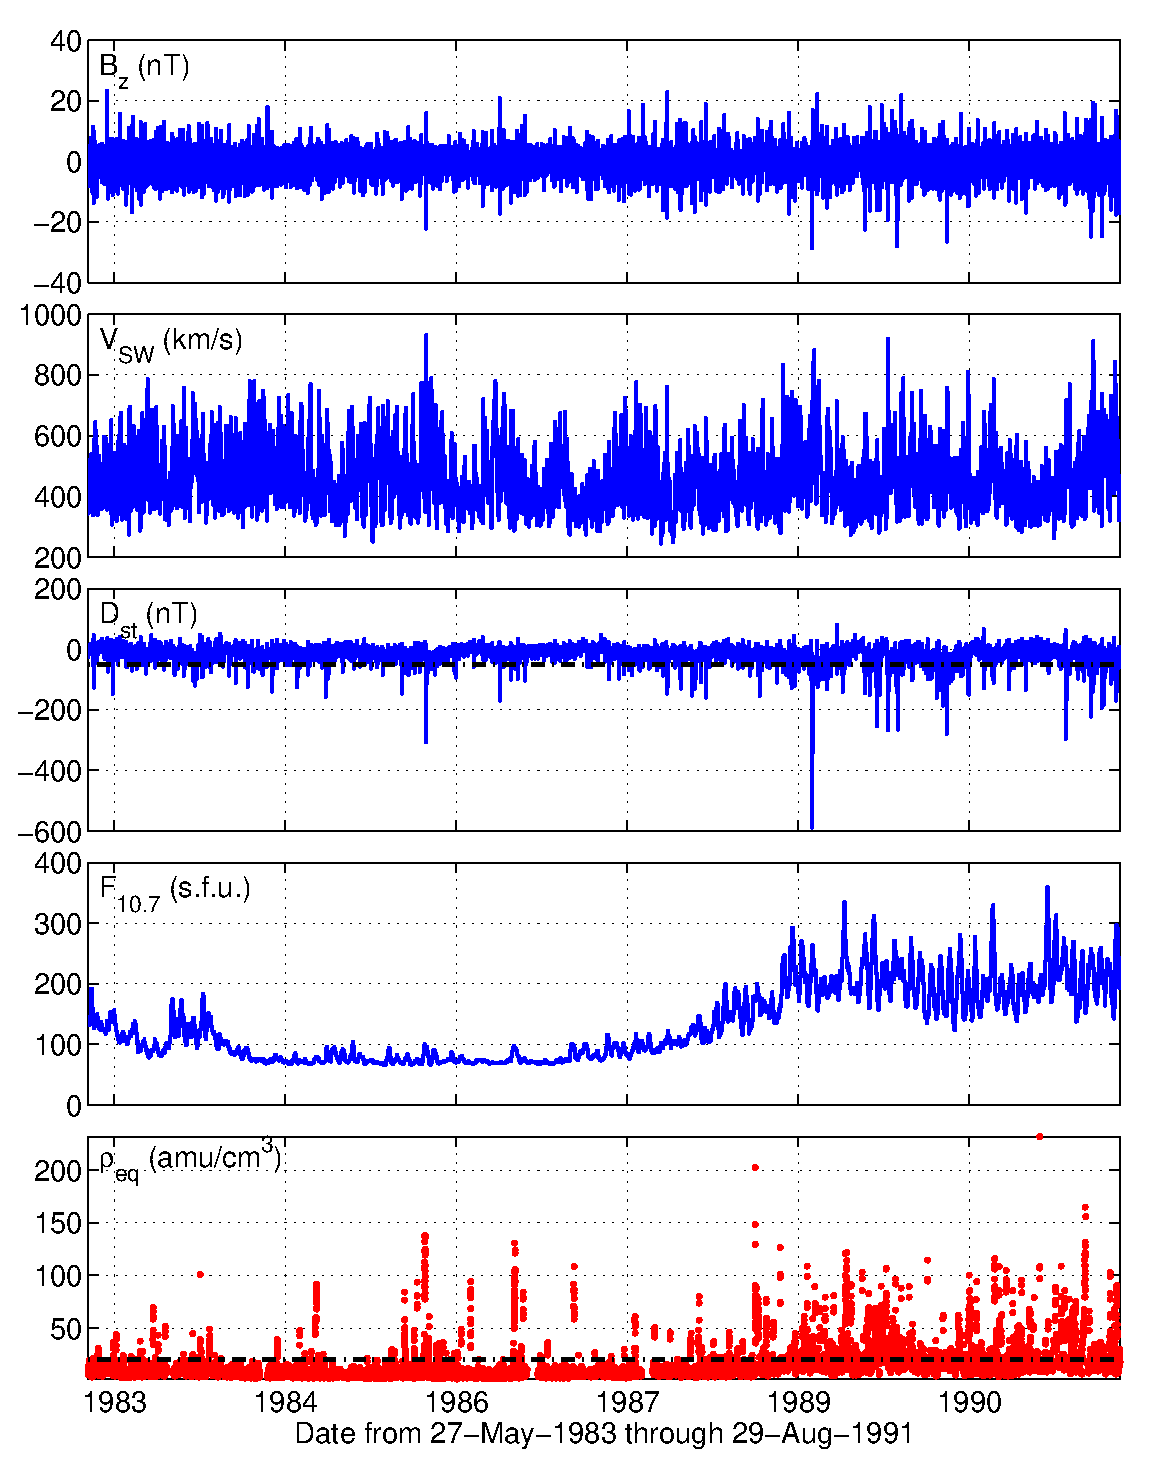
\includegraphics[scale=0.45]{UsedFigures/2016SW001507R-p01.eps}
	\caption{Overview of data used in this article. The top four panels show parameters from \citet{Kondrashov2014ReconstructionOfGaps} and the bottom panel contains $\rho_{eq}$ based on GOES 6 measurements from \citet{Denton} after interpolation and averaging described in the text. Dashed horizontal lines in the $D_{st}$ and $\rho_{eq}$ panels indicate sample event cutoff thresholds of $D_{st} = -50$~nT and $\rho_{eq} = 20$~amu/cm$^3$ considered in Section~3.}
	\label{fig:AllData}
\end{figure}

\clearpage

\begin{figure}[htp!]
	\centering
	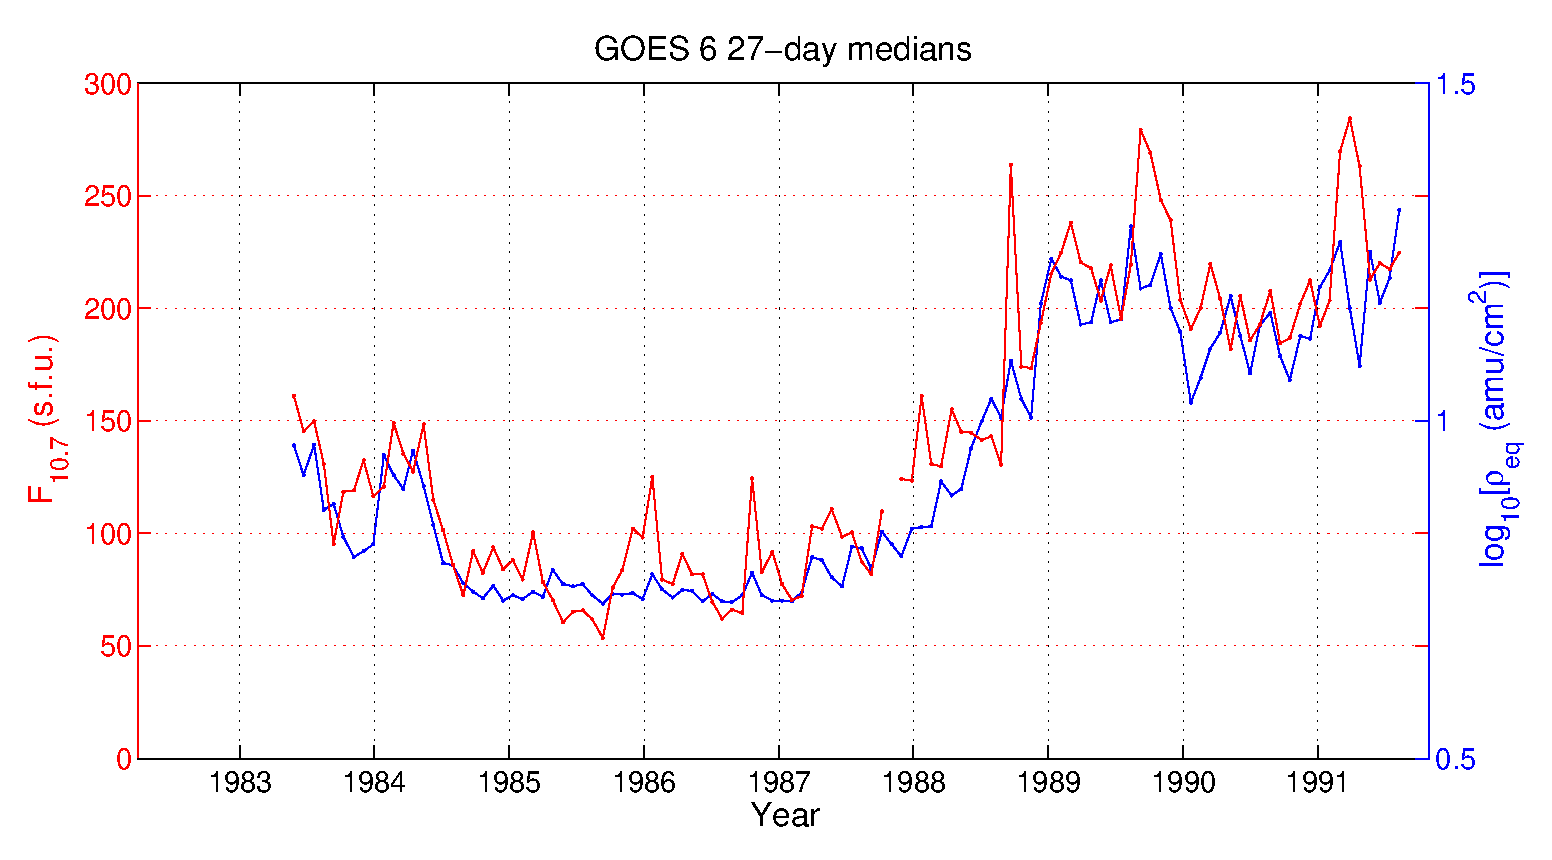
\includegraphics[scale=0.40]{UsedFigures/2016SW001507R-p02a.eps}
	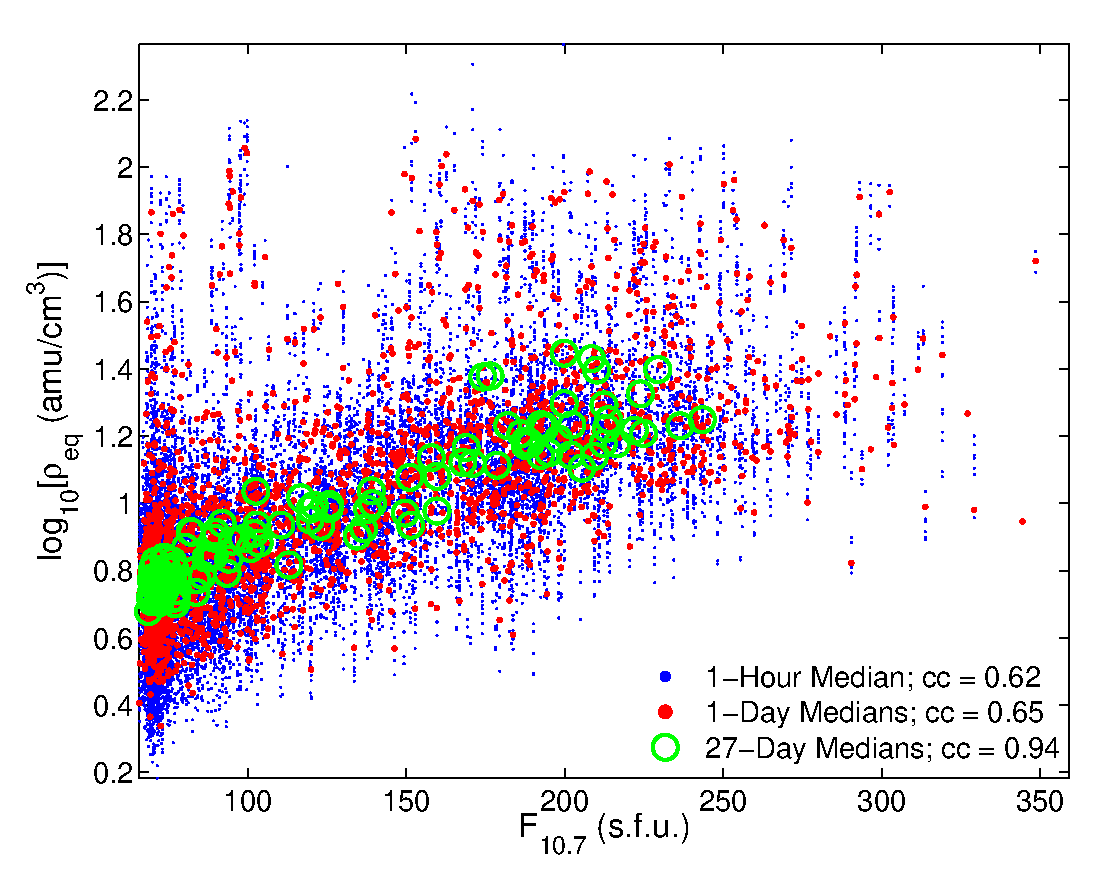
\includegraphics[scale=0.40]{UsedFigures/2016SW001507R-p02b.eps}
	\caption{Top: 27-day non-overlapping medians of $F_{10.7}$ and $\log_{10}(\rho_{eq})$ from GOES 6. Bottom: Scatter plot of $\log_{10}(\rho_{eq})$ and $F_{10.7}$ using medians in non-overlapping hour, day, and 27-day windows.}
	\label{fig:ccplot}
\end{figure}
\clearpage

\begin{figure}[h]
	\centering
	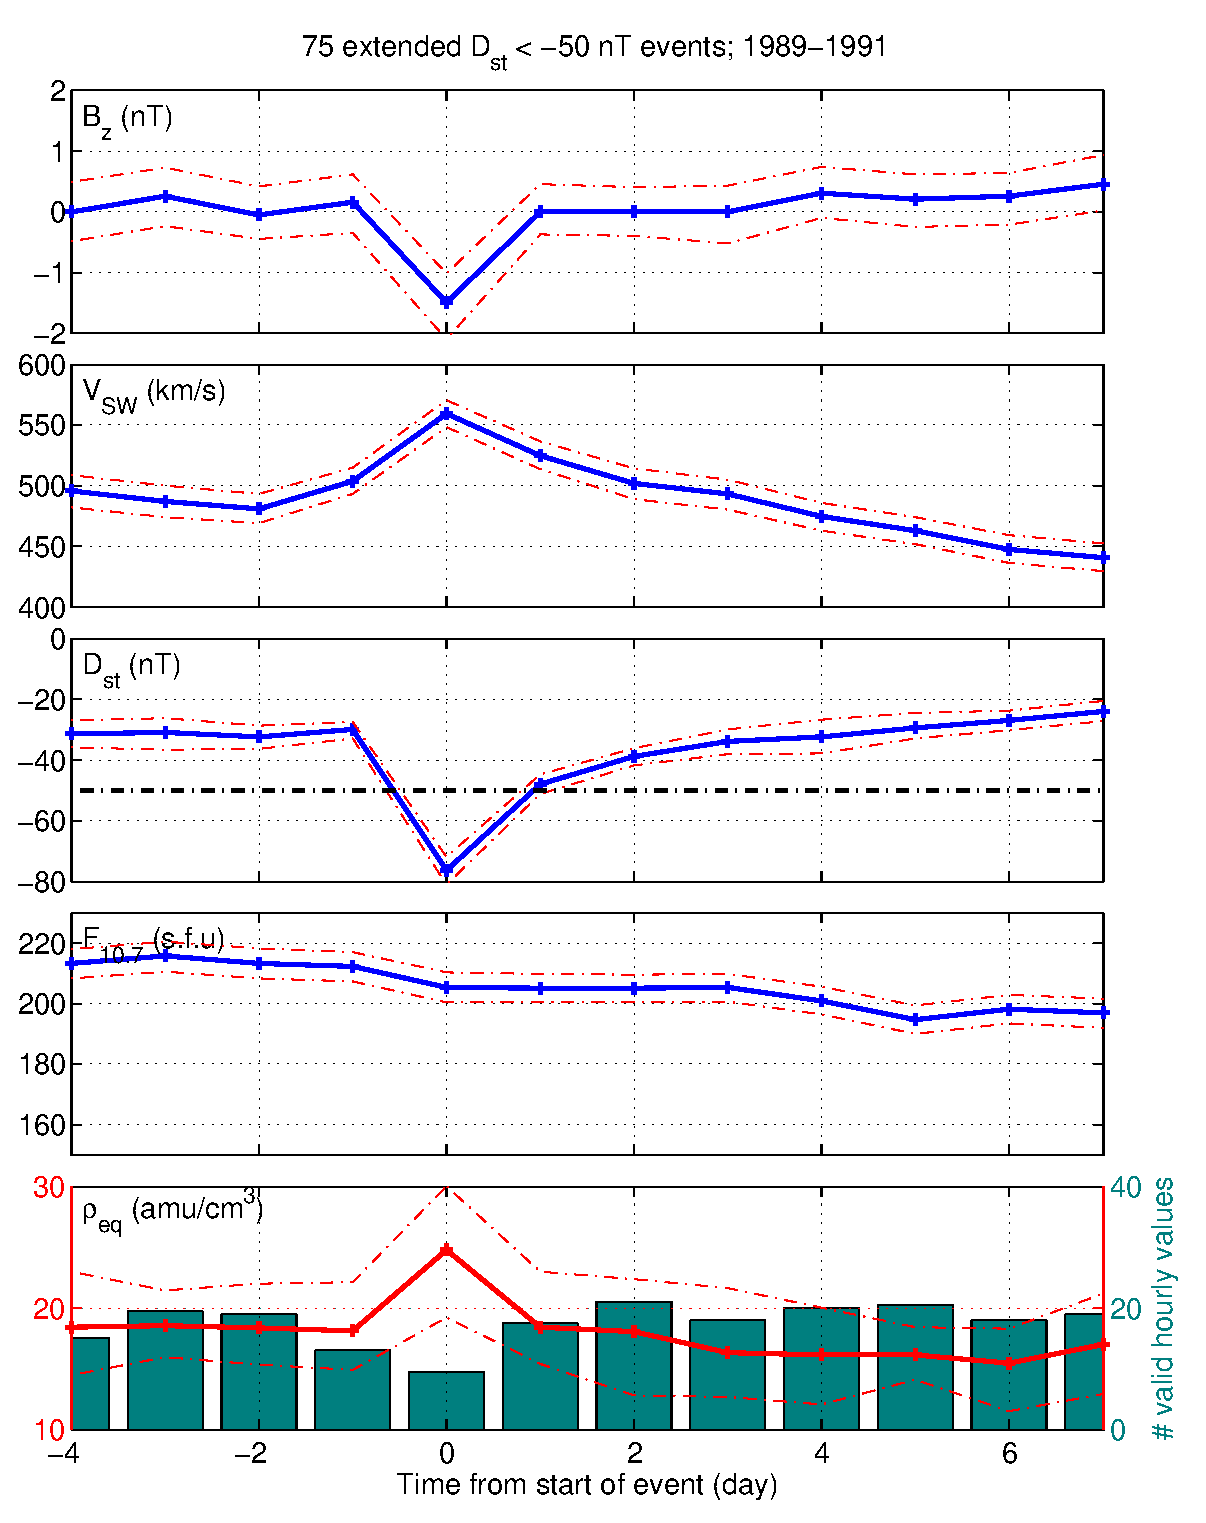
\includegraphics[scale=0.40]{UsedFigures/2016SW001507R-p03a.eps}
	\\
	\rule[1ex]{5cm}{1pt}
	\\
	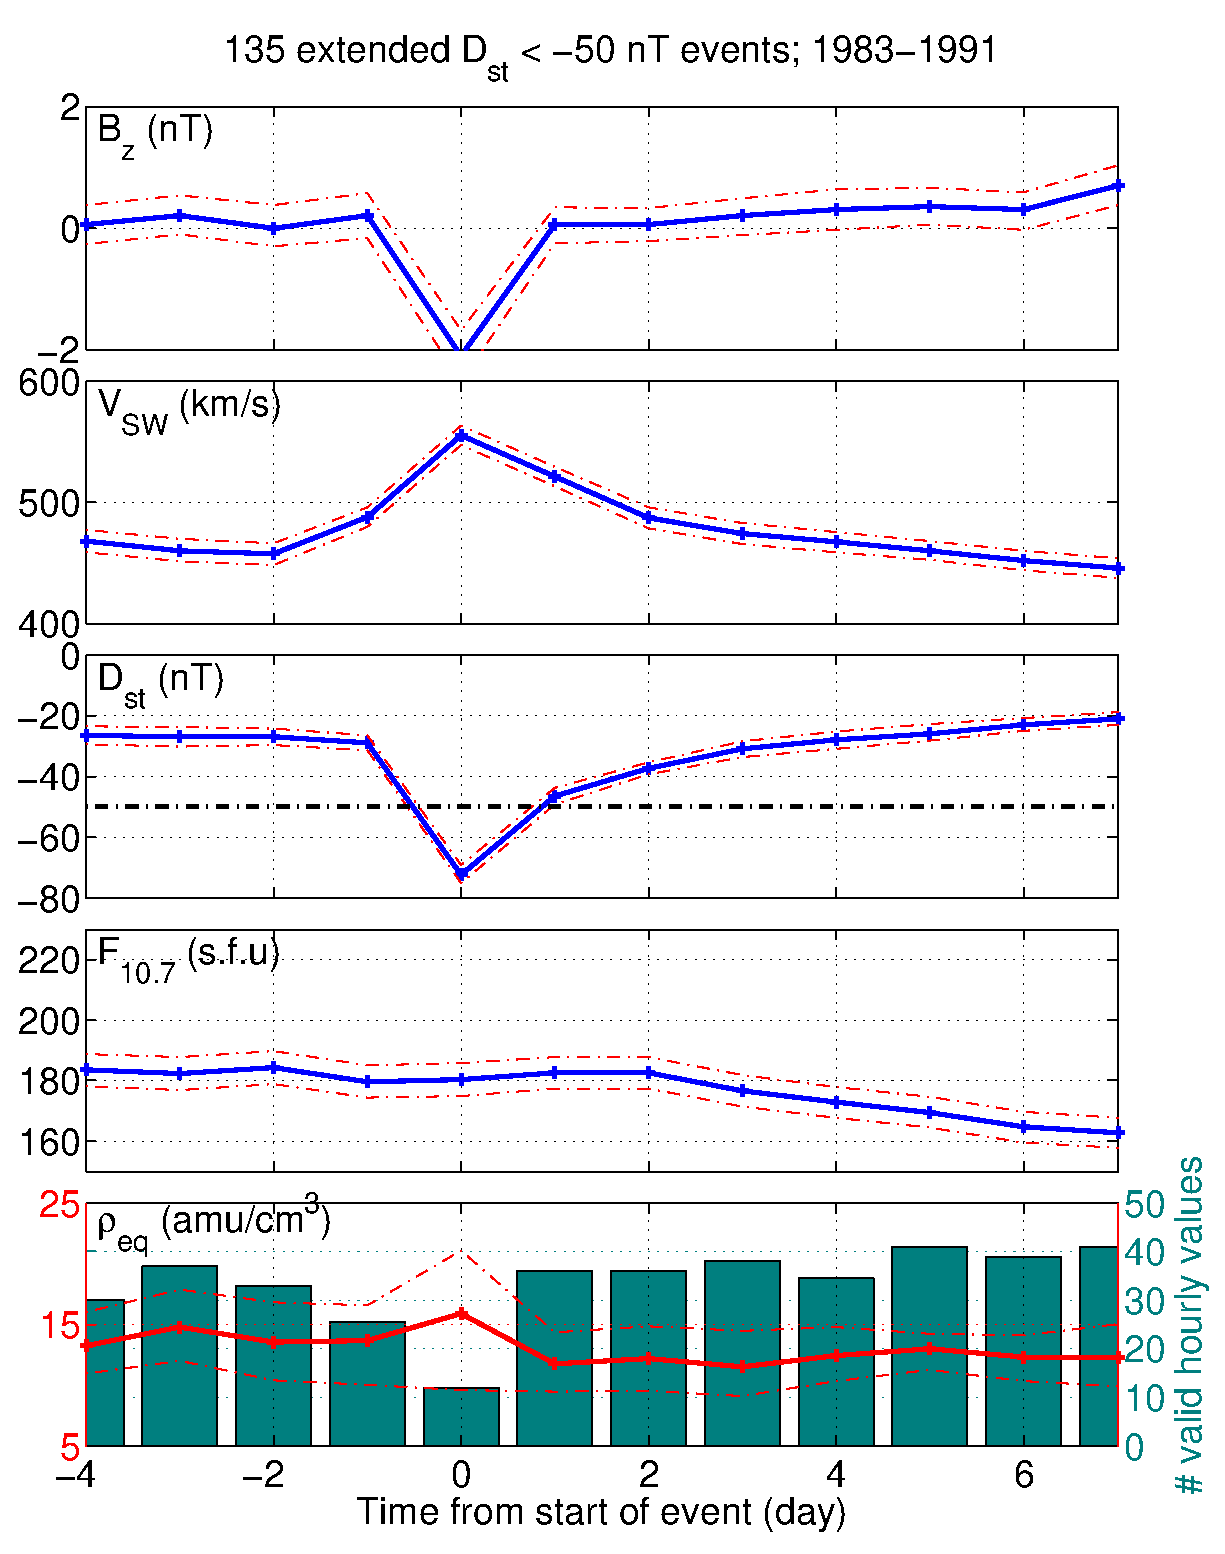
\includegraphics[scale=0.40]{UsedFigures/2016SW001507R-p03b.eps}
	\caption{$D_{st}$ events from GOES 6 using daily medians. Top: Events in the interval 1989-1991; compare to \citet{Takahashi2010} Figure~11. Bottom: Events in the interval 1983-1991.}
	\label{fig:DailyAveragedDstEvents}
\end{figure}

\clearpage

\begin{figure}[tp!]
	\centering
	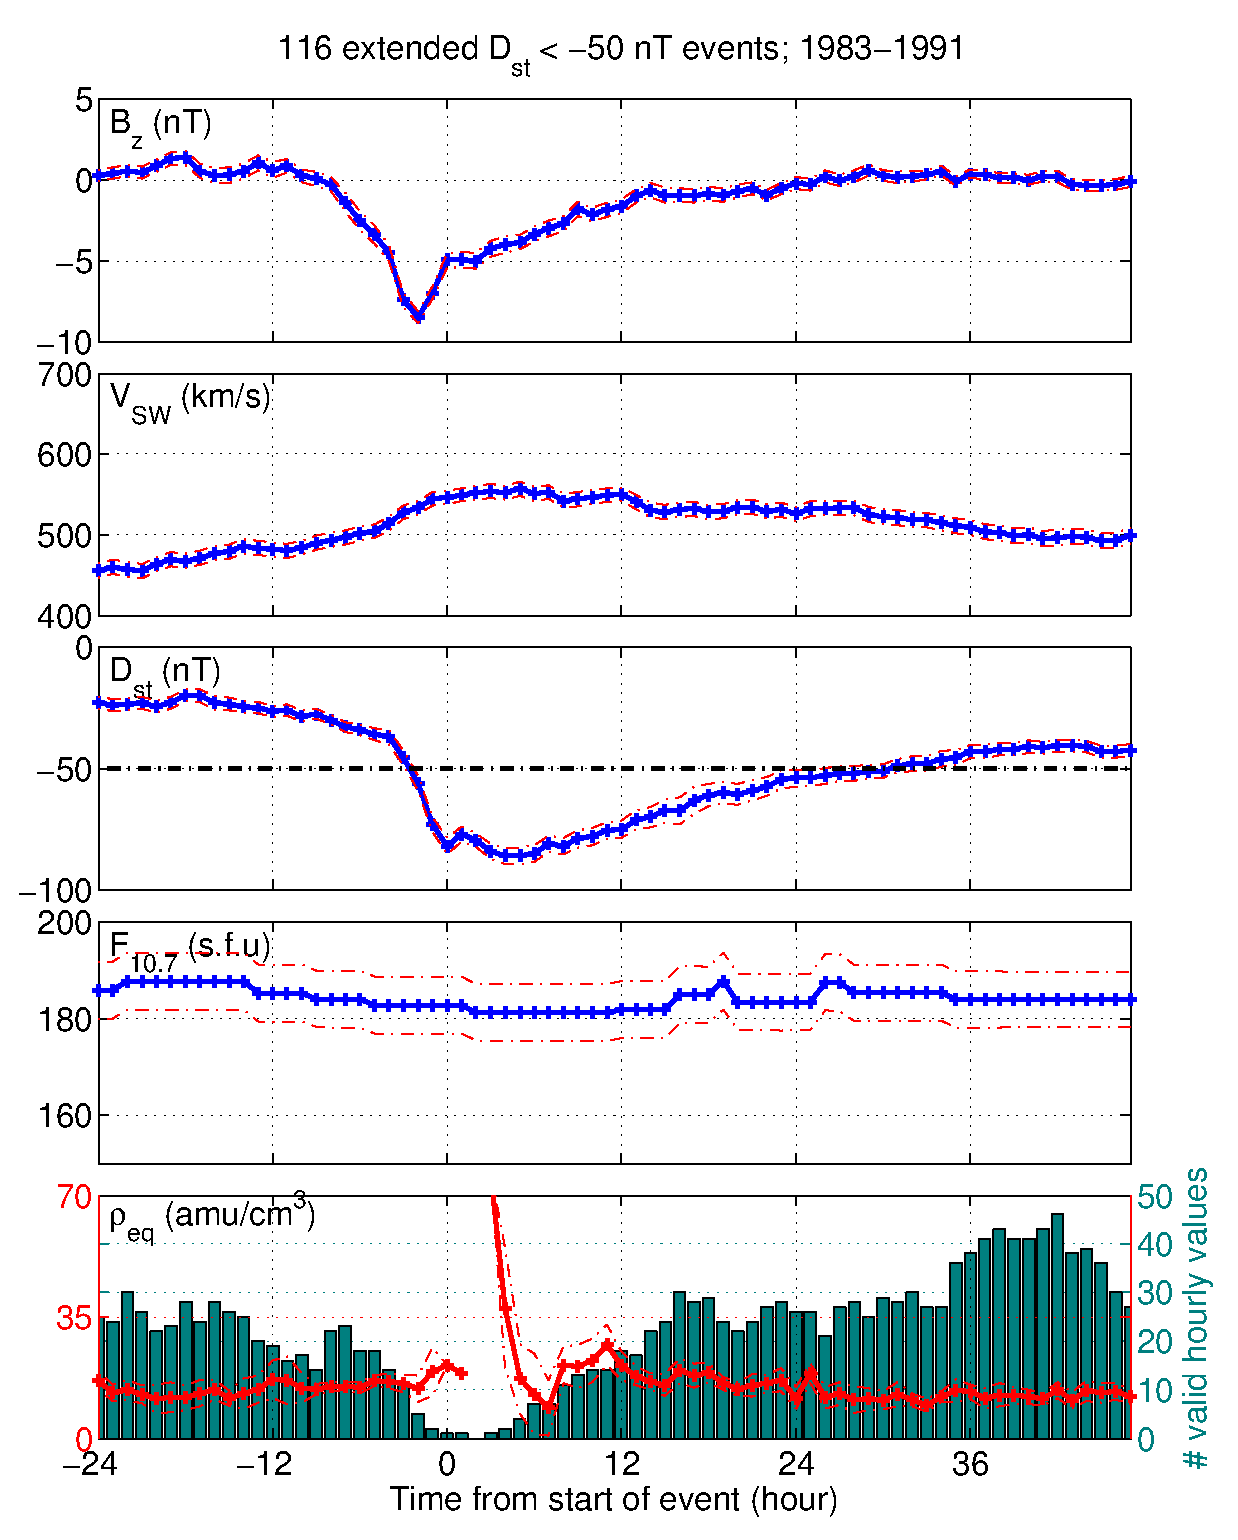
\includegraphics[scale=0.40]{UsedFigures/2016SW001507R-p04a.eps}
	\\
	\rule[1ex]{5cm}{1pt}
	\\
	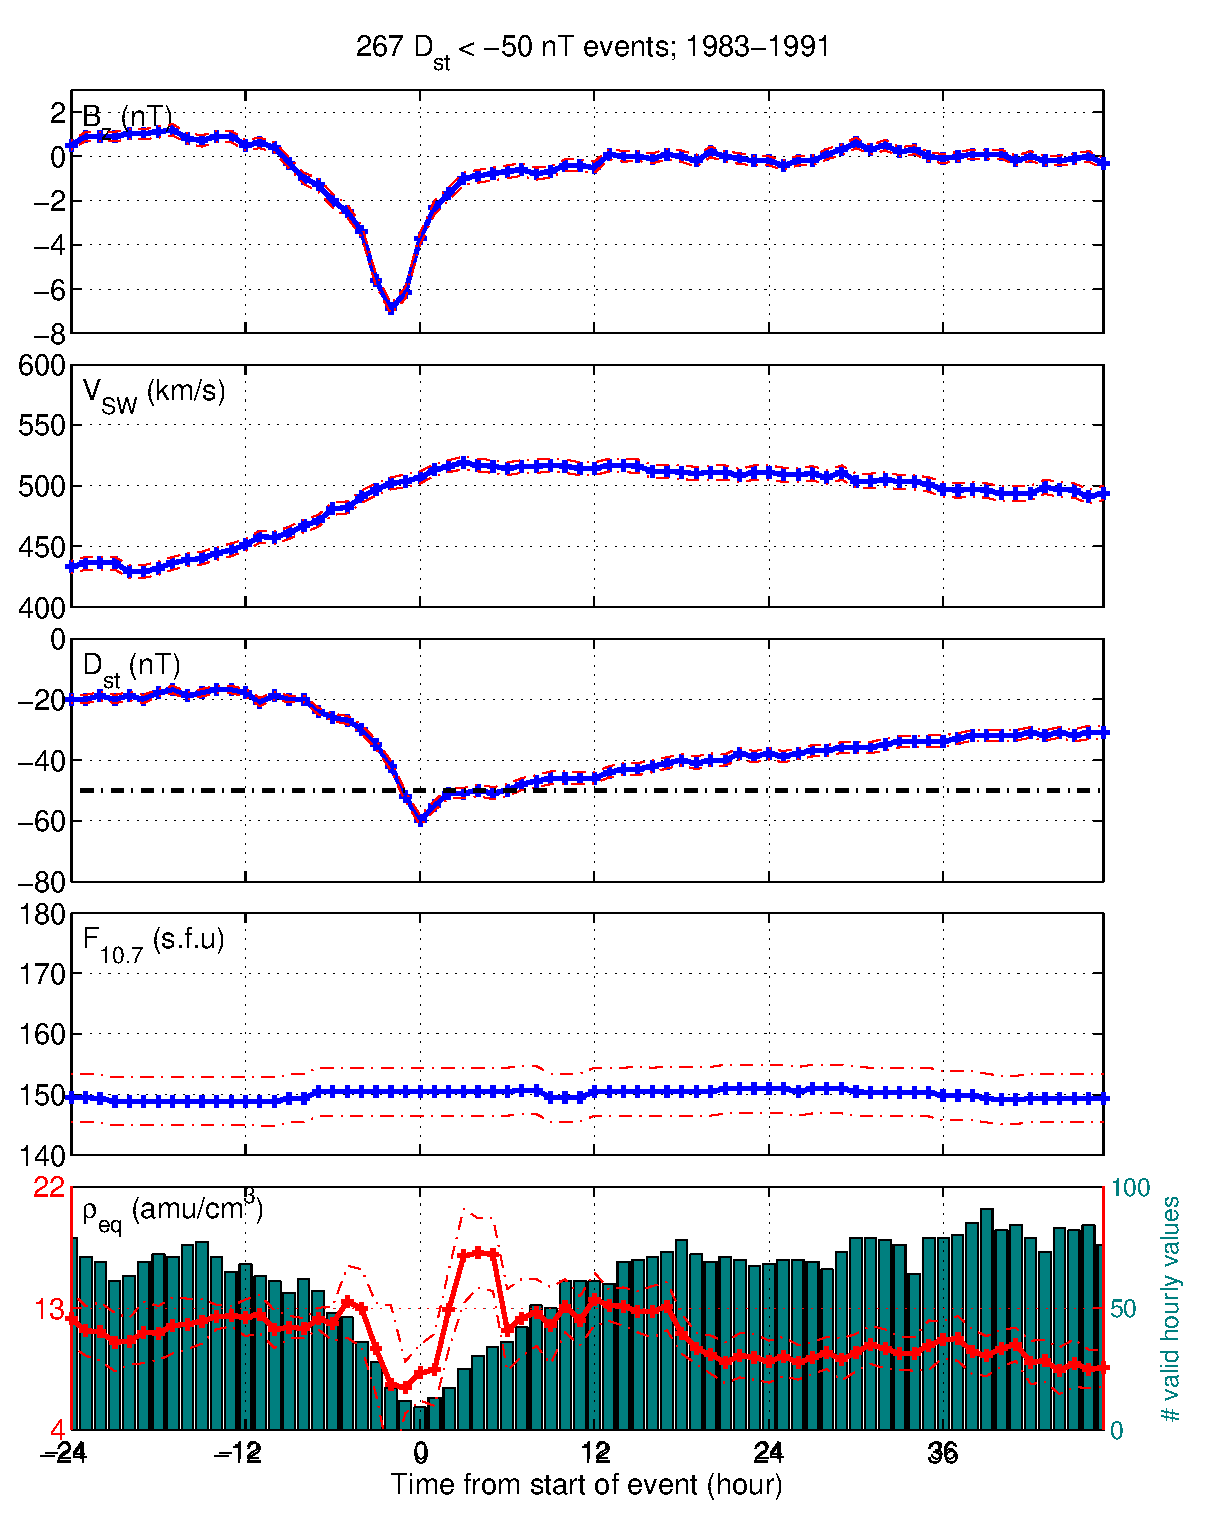
\includegraphics[scale=0.40]{UsedFigures/2016SW001507R-p04b.eps}
	\caption{$D_{st}$ events from GOES 6 using hourly medians. Top: Events with the constraint that $D_{st}$ stayed below $-50$~nT for at least 12~hours after crossing below $-50$~nT.  Bottom: Same as Top except without constraint.}
	\label{fig:HourlyAveragedDstEvents}
\end{figure}

\clearpage
\begin{figure}[tp!]
	\centering
	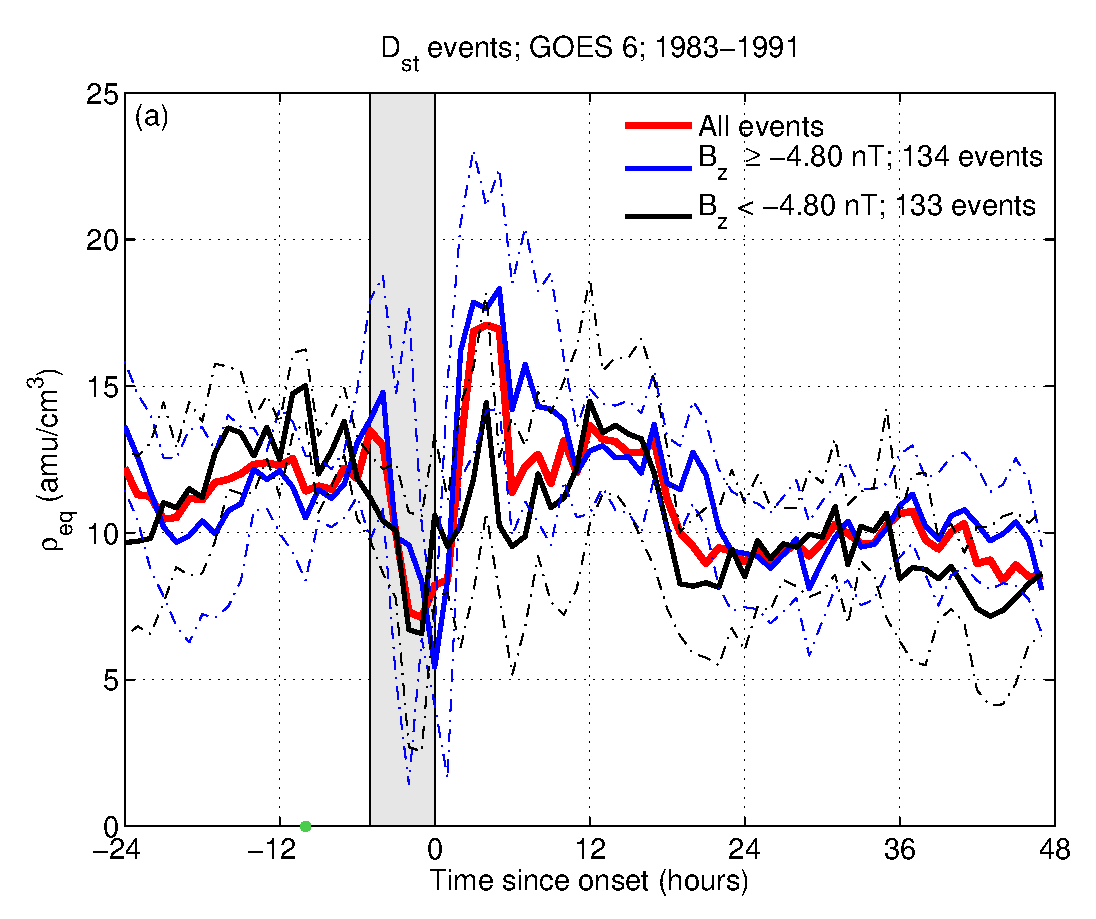
\includegraphics[scale=0.40]{UsedFigures/2016SW001507R-p05a.eps}
	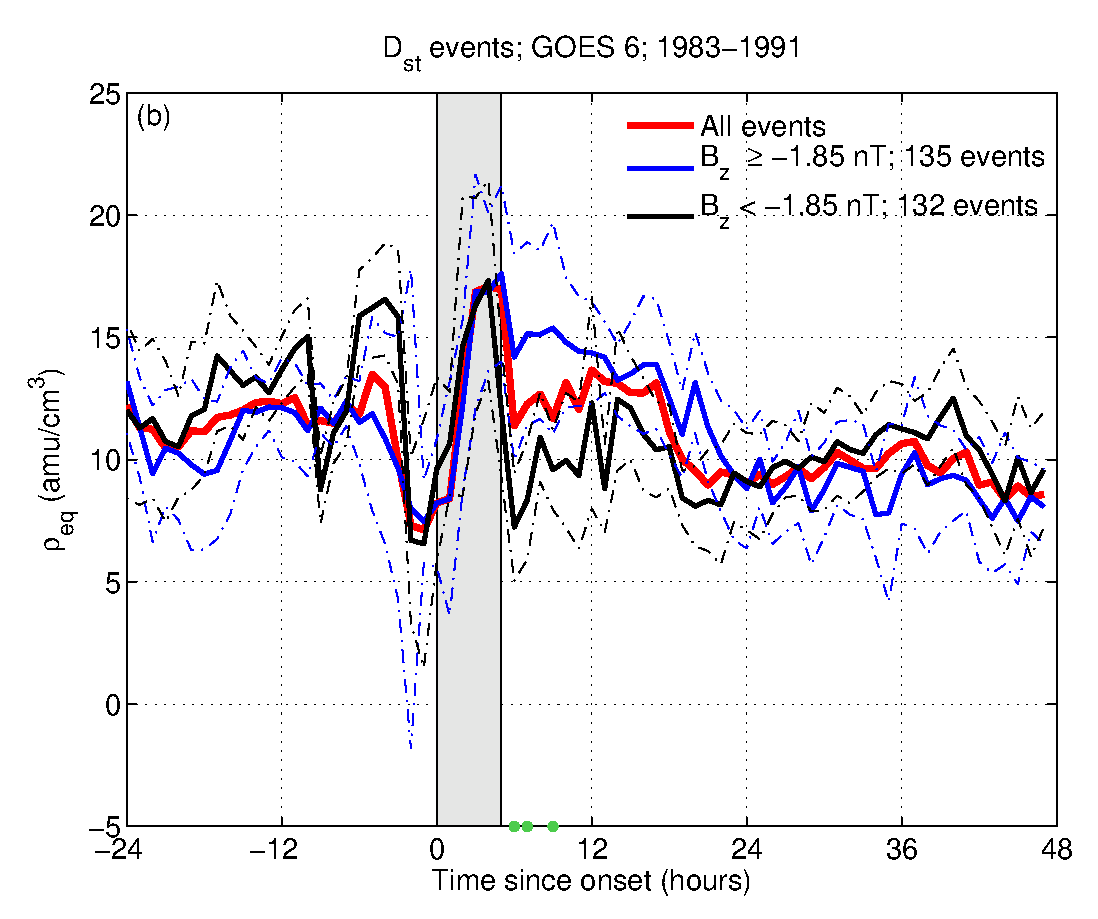
\includegraphics[scale=0.40]{UsedFigures/2016SW001507R-p05b.eps}
	\caption{$D_{st}$ events of the bottom panel of Figure~\ref{fig:HourlyAveragedDstEvents} separated by the average $D_{st}$ value (a) at onset and four hours before, and (b) at onset and four hours after.}
	\label{fig:BzBinnedDstEvents}
\end{figure}

\begin{figure}[tp!]
	\centering
	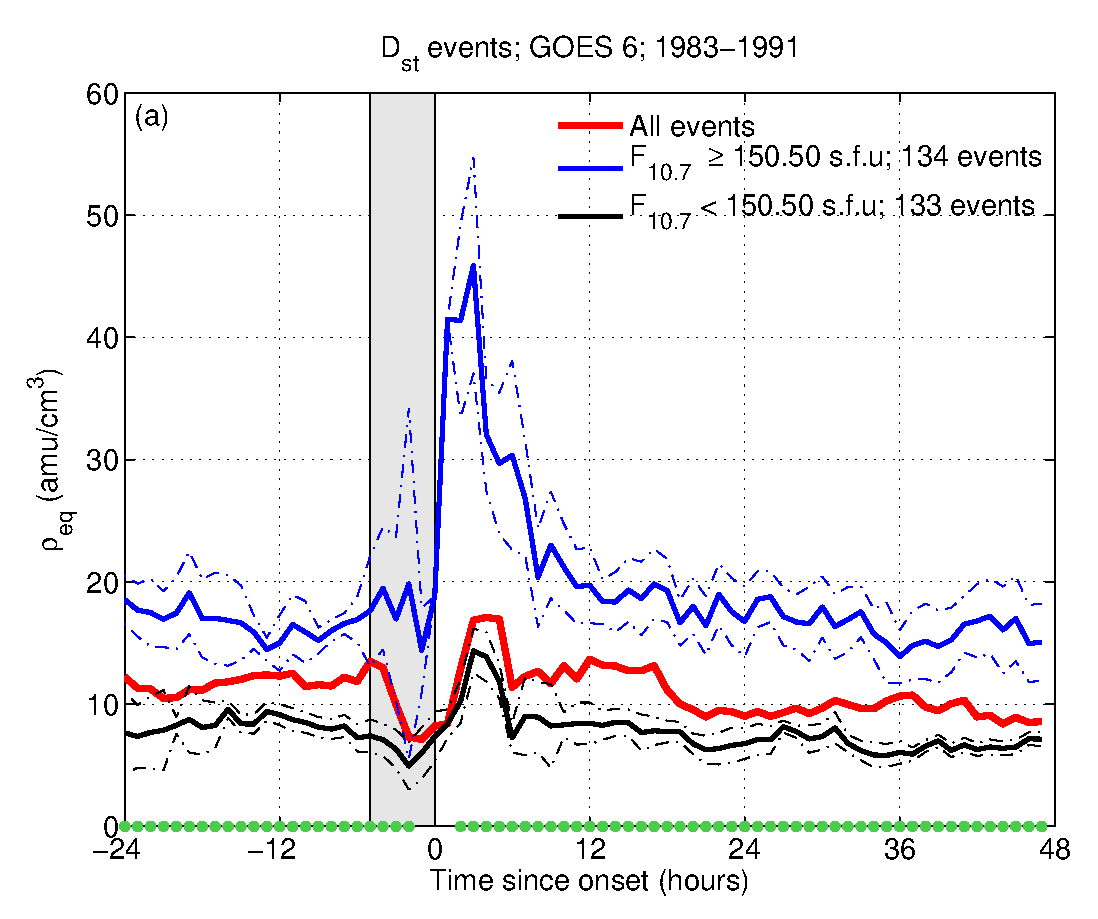
\includegraphics[scale=0.40]{UsedFigures/2016SW001507R-p06a.eps}
	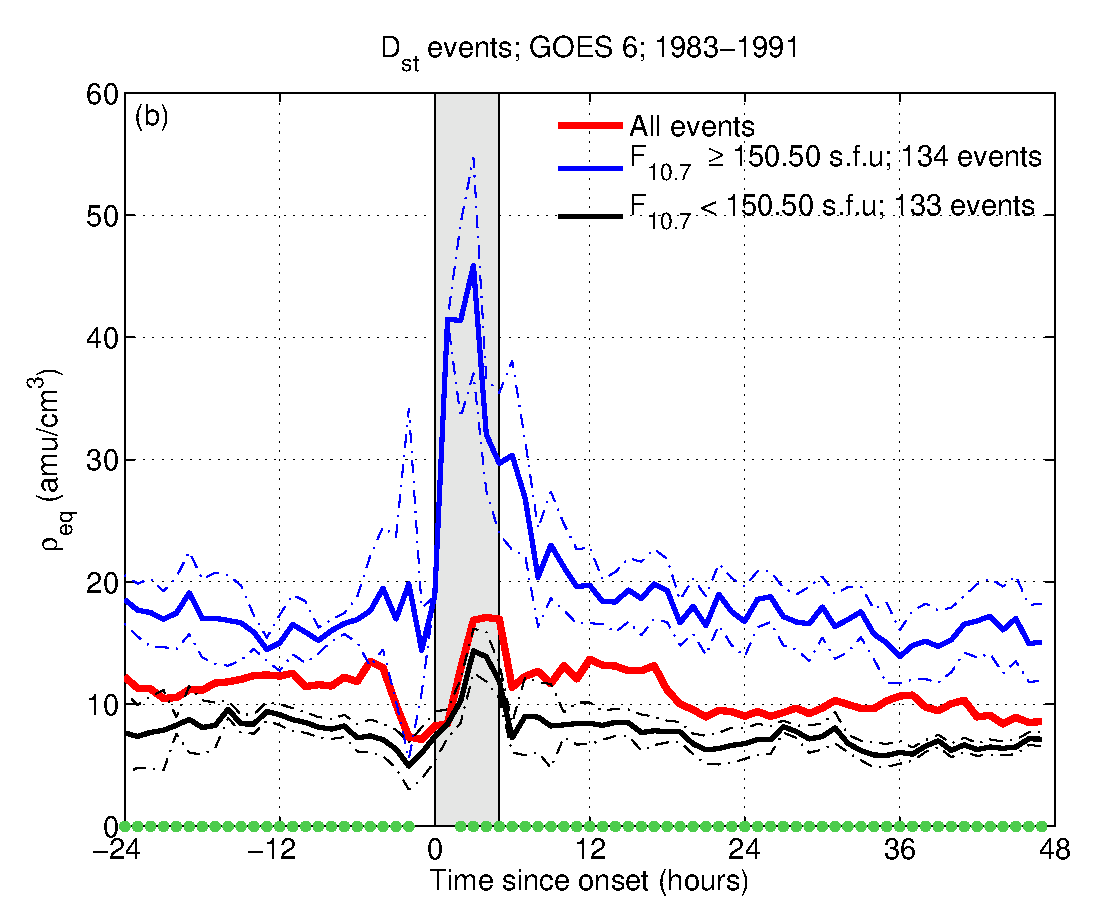
\includegraphics[scale=0.40]{UsedFigures/2016SW001507R-p06b.eps}
	\caption{$D_{st}$ events of the bottom panel of Figure~\ref{fig:HourlyAveragedDstEvents} separated by the average $F10.7$ value (a) at onset and four hours before, and (b) at onset and four hours after.}
	\label{fig:F107BinnedDstEvents}
\end{figure}

\clearpage

\begin{figure}[htp!]
	\centering
	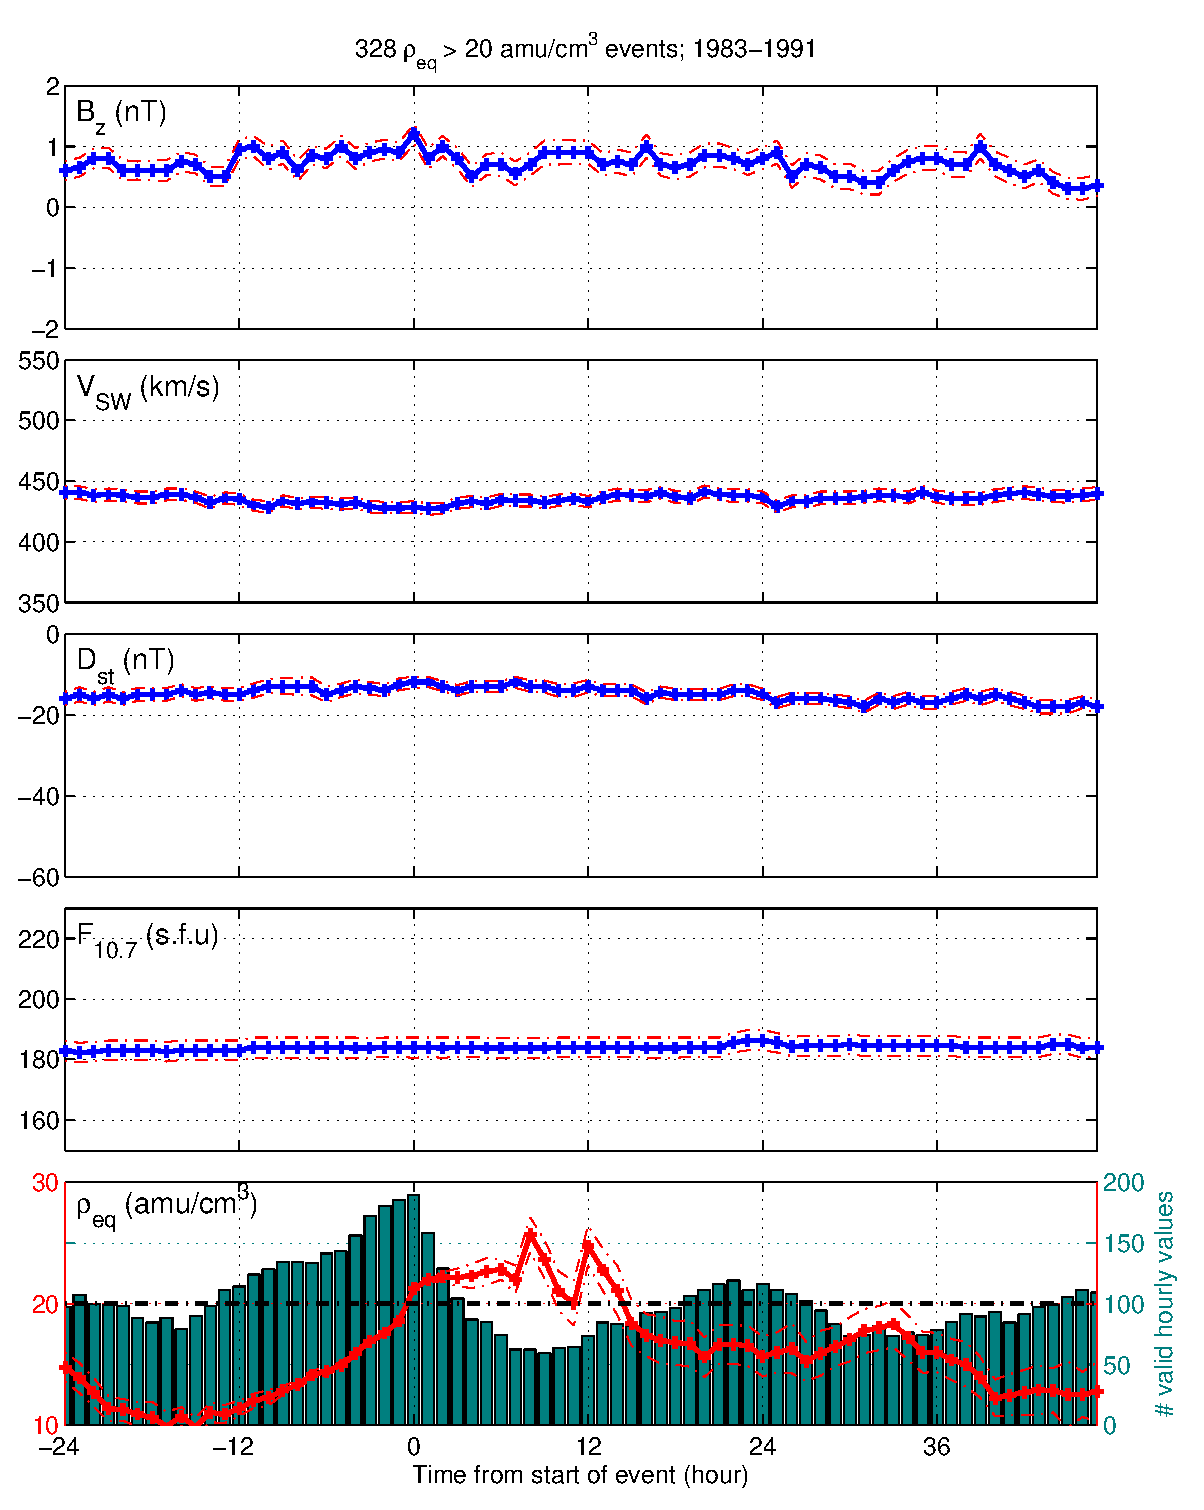
\includegraphics[scale=0.40]{UsedFigures/2016SW001507R-p07.eps}
	\caption{$\rho_{eq} >$ 20~amu/cm$^3$ events from GOES 6 using hourly medians.}
	\label{fig:HourlyAveragedRhoEvents}
\end{figure}

\clearpage
\begin{figure}[tp!]
	\centering
	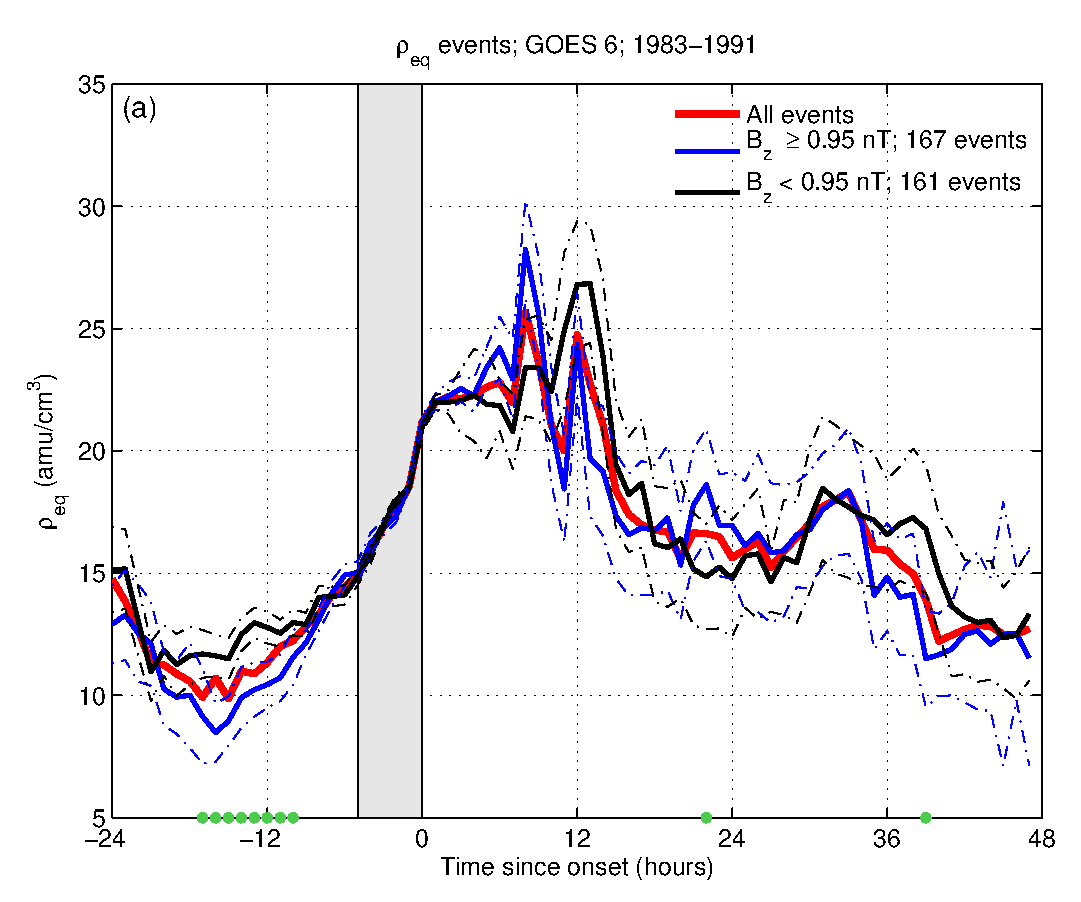
\includegraphics[scale=0.40]{UsedFigures/2016SW001507R-p08a.eps}
	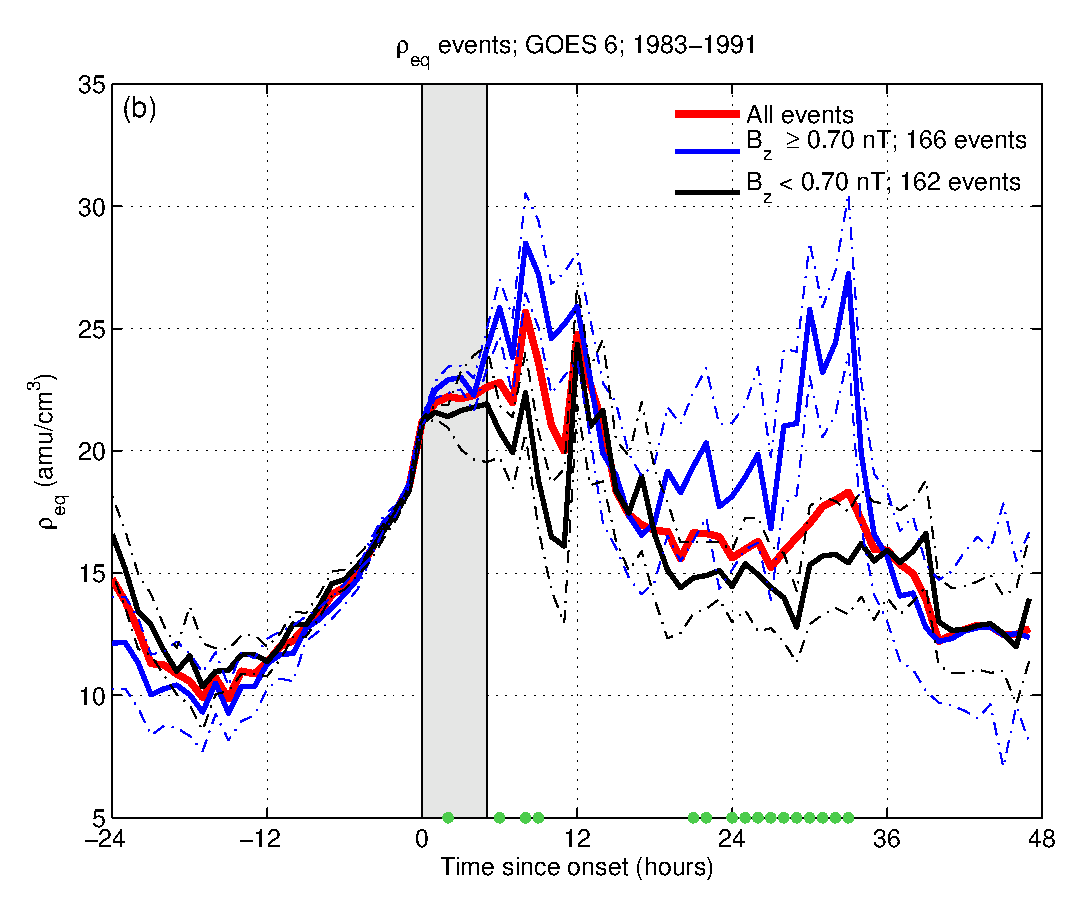
\includegraphics[scale=0.40]{UsedFigures/2016SW001507R-p08b.eps}
	\caption{$\rho_{eq}$ events of Figure~\ref{fig:HourlyAveragedRhoEvents} separated by the average $B_z$ value (a) at onset and four hours before, and (b) at onset and four hours after.}
	\label{fig:BzBinned}
\end{figure}

\begin{figure}[tp!]
	\centering
	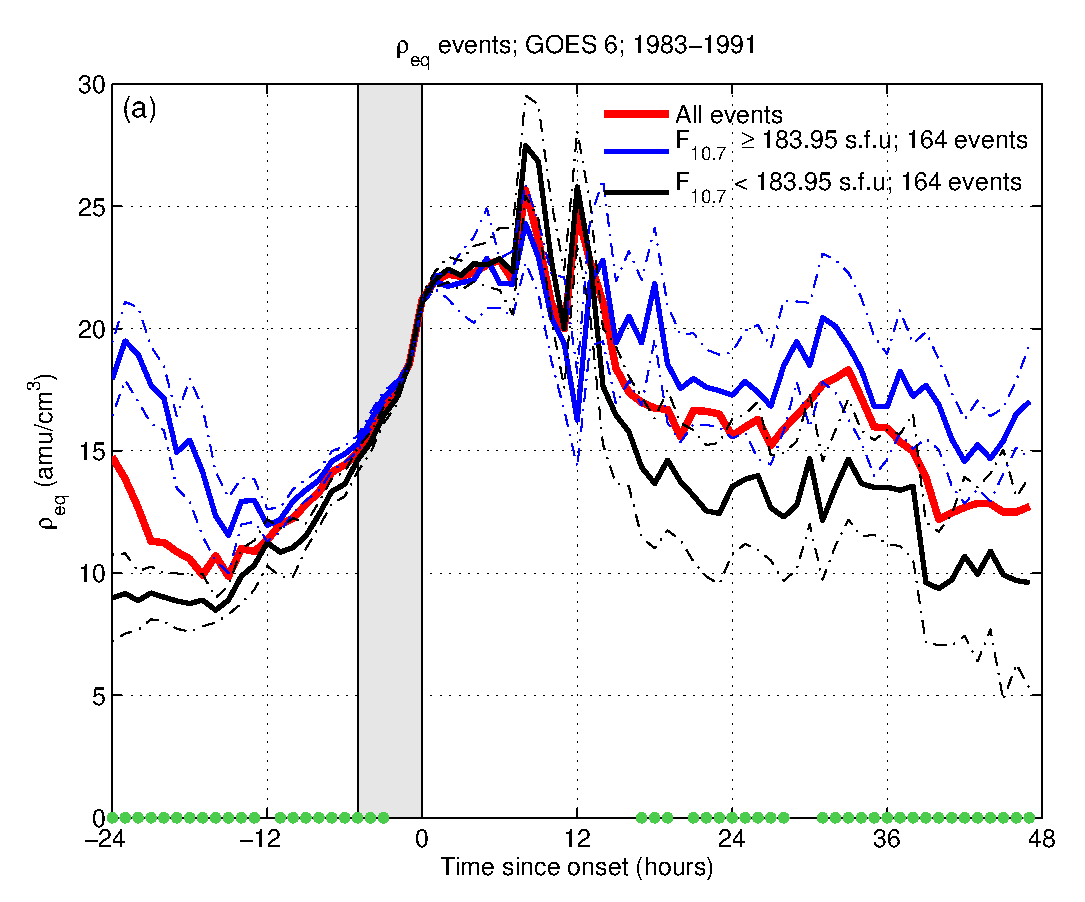
\includegraphics[scale=0.40]{UsedFigures/2016SW001507R-p09a.eps}
	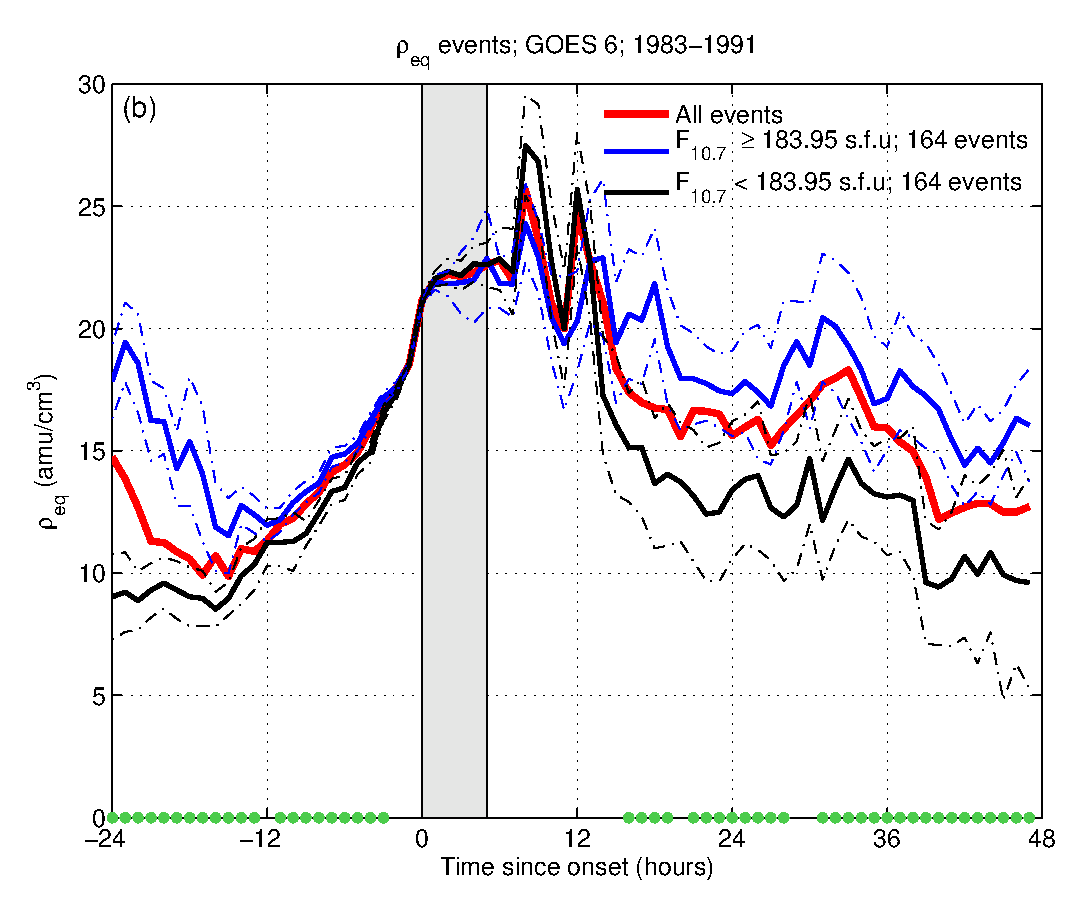
\includegraphics[scale=0.40]{UsedFigures/2016SW001507R-p09b.eps}
	\caption{$\rho_{eq}$ events of Figure~\ref{fig:HourlyAveragedRhoEvents} separated by the average $F10.7$ value (a) at onset and four hours before, and (b) at onset and four hours after.}
	\label{fig:F107Binned}
\end{figure}

\end{document}



